
\section{Desarrollo del trabajo}  

\label{desarrollo}
En esta sección se va a proceder a explicar el desarrollo de este trabajo. Se va a dividir en seis partes:
\begin{itemize}
    \item Preprocesamiento de los datos.
    \item Procesamiento de los datos: Creación de modelos.
    \item MLOps: monitorización y automatización del proceso.
    \item Comparativa de modelos.
    \item Almacenamiento de los datos.
    \item Visualización de los datos.
\end{itemize}

Para tener los pasos mejor pautados, véase la Figura \ref{arquitectura} en donde se muestra la arquitectura del proyecto. También se puede ver de una manera más clara y visual cómo están conectadas las tecnologías explicadas en el apartado anterior.
\begin{figure}[H]
    \centering
    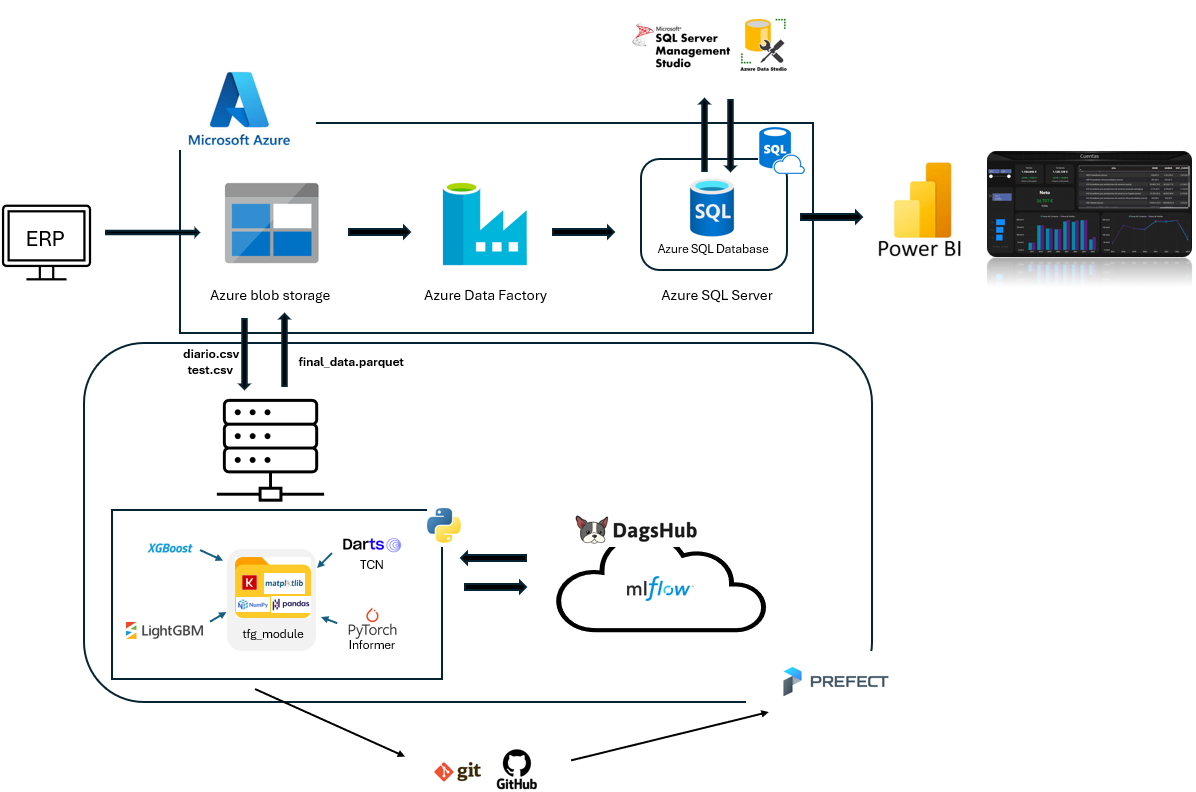
\includegraphics[scale = 0.6]{imgs/Arquitectura.png}
    \caption{Arquitectura software del proyecto.}
    \label{arquitectura}
\end{figure}

Cada sección de la Figura \ref{arquitectura} se va a explicar más en detalle a lo largo de este apartado.  No obstante, se ve apropiado comentarla por encima. Todo empieza en Azure Blob Storage donde los archivos (\Code{.csv} en este caso) están almacenados. Estos archivos contienen datos contables y se dividen de esta manera de tal forma que \Code{diario.csv} serán los datos contables empleados para entrenamiento y validación y \Code{test.csv} para testeo utilizados por los algoritmos de aprendizaje automático.

Una vez establecido el punto de partida, un servidor (en caso de este trabajo lo simula el propio ordenador) recoge estos archivos \Code{.csv} para preprocesarlos, procesarlos y  generar predicciones con los cuatro algoritmos mencionados en la sección 2. Estas predicciones son a partir de series temporales de Compras y Ventas, obtenidas en el preprocesamiento de los datos.


Los modelos generados a partir de los algoritmos son almacenados en Mlflow. Concretamente en un repositorio de Dagshub en la nube. De esta manera se tiene un control y seguimientos del proceso de aprendizaje automático. Una vez se tienen los modelos ahí, se eligen a los mejores modelos de cada algoritmo para poder compararlos y elegir al mejor y utilizar sus predicciones para posteriormente poder mostrarlas. Esto se resume en el archivo  \Code{final\_data.parquet} que contiene los datos a utilizar por Power BI.

Este \Code{.parquet} se envía en nuevo a Azure Blob Storage, en donde Azure Data Factory, se encargará de copiar estos datos a una tabla en una base de datos SQL. Será de este origen de donde Power BI extraiga los datos para posteriormente crear las visualizaciones.

Algo \ul{muy importante} a mencionar es que  todo el desarrollo y de más relacionado con este trabajo está alojado en un repositorio de \href{https://github.com/JCOQUE/TFG-ingenieria.git}{Github}\fn{https://github.com/JCOQUE/TFG-ingenieria.git}. Ahí se puede ver e indagar más en detalle en el desarrollo de este trabajo; más allá de lo que se va a comentar en esta sección. Además, contiene un README.md que se recomienda leer para un entendimiento más profundo del contenido del repositorio; así como de claves en el desarrollo de este trabajo.

\subsection{Preprocesamiento de los datos}
Los algoritmos de aprendizaje automático necesitan un preprocesamiento de los datos previo para hacer un entrenamiento eficiente y, de esta manera, obtener un resultado lo más preciso posible. Como punto de partida, véase la Figura \ref{preprocesamiento}.
\begin{figure}[H]
    \centering
    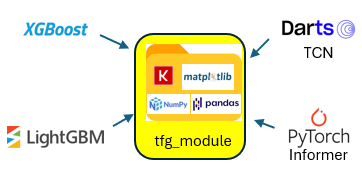
\includegraphics[width = 0.48\textwidth]{imgs/Preprocesamiento.png}
    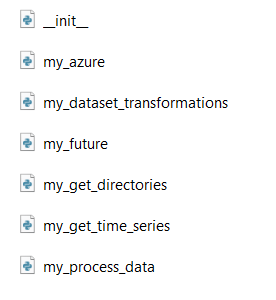
\includegraphics[scale = 0.9]{imgs/contenido_tfg_module.png}
    \caption{Carpeta tfg\_module (izquierda) junto a su contenido (derecha).}
    \label{preprocesamiento}
\end{figure}

En la Figura \ref{preprocesamiento} se puede ver a la izquierda la carpeta "tfg\_module". Esta se trata de un módulo de Python creado por el autor para el desarrollo de este trabajo. A la derecha de la Figura \ref{preprocesamiento} se puede ver el contenido de este módulo. En él hay un archivo \Code{\_\_init\_\_.py}. Esto se trata de una nomenclatura del propio lenguaje de programación de Python que indica que esta carpeta es un módulo de Python y que, por tanto, tiene un comportamiento distinto al de una carpeta normal. El resto del  contenido son archivos \Code{.py}, cada uno con un objetivo distinto. 

Este módulo hace muchas cosas, pero las \ti{más importantes} son:
\begin{itemize}
	\item Extraer (\ti{pull}) y enviar (\ti{push}) archivos de Azure Blob Storage vía API (\Code{my\_azure.py}).
	\item Preprocesa los datos para añadir columnas (e.g. Compras y Ventas) a partir de las ya existentes (\Code{my\_dataset\_transformations.py}).
	\item Una vez preprocesados los datos, se encarga de transformarlos a una serie temporal de Compras (o de Ventas, según se indique). Esto quiere decir que se obtiene un \ti{DataFrame} únicamente con una columna \Code{Fecha} y otra \Code{Compras}. De esto se encarga \Code{my\_get\_time\_series.py}.
	\item También es encarga de generar las fechas futuras sobre las que se va a predecir, así como de almacenar estas predicciones en un \ti{DataFrame} para posteriormente poder almacenarlas en un \Code{.csv}. De esto se encarga \Code{my\_future.py}.
\end{itemize}

Todas estas funcionalidades son comunes a los algoritmos de aprendizaje automático empleados en el trabajo. Además de lo comentado recientemente, este módulo aporta una característica fundamental al desarrollo de código: abstraer funcionalidad  para cada distinto algoritmo de aprendizaje automático. Con esto se consigue un código más limpio por tres motivos: el primero es porque, de esta manera, el código de los algoritmos se centra en eso: en los algoritmos. Toda la parte de preparación de datos se lleva por detrás en este módulo. El segundo es que, debido a que cada algoritmo pertenece a una librería distinta (XGBoost, LightGBM, Darts y PyTorch), cada uno tiene sus peculiaridades y su manera de preprocesar los datos, entrenarlos y obtener resultados. Con  este módulo lo que se consigue es que el código de cada algoritmo sea muy similar al del resto, pues estas diferencias de librerías se tienen en cuenta en el módulo y no en el código de los algoritmos en sí. En otras palabras, \B{se consigue estandarizar}, en la medida de lo posible, el código de los cuatro algoritmos de aprendizaje automático. Por último, se consigue una reutilización de código eficiente, cumpliendo así con un principio de programación fundamental: \ti{Don't repeat yourself} (DRY).

Para ver un ejemplo visual de lo que se acaba de mencionar, véase la Figura \ref{ejAbstraccion} en donde \Code{my\_process\_data.py} del módulo creado tiene en cuenta si tiene que procesar\fnm\ los datos para el algoritmo Informer o cualquier otro.
\fnt{Este módulo principalmente se encarga de preprocesamiento de los datos, pero también cumple con algunas funcionalidades de procesamiento.}
\begin{figure}[H]
    \centering
    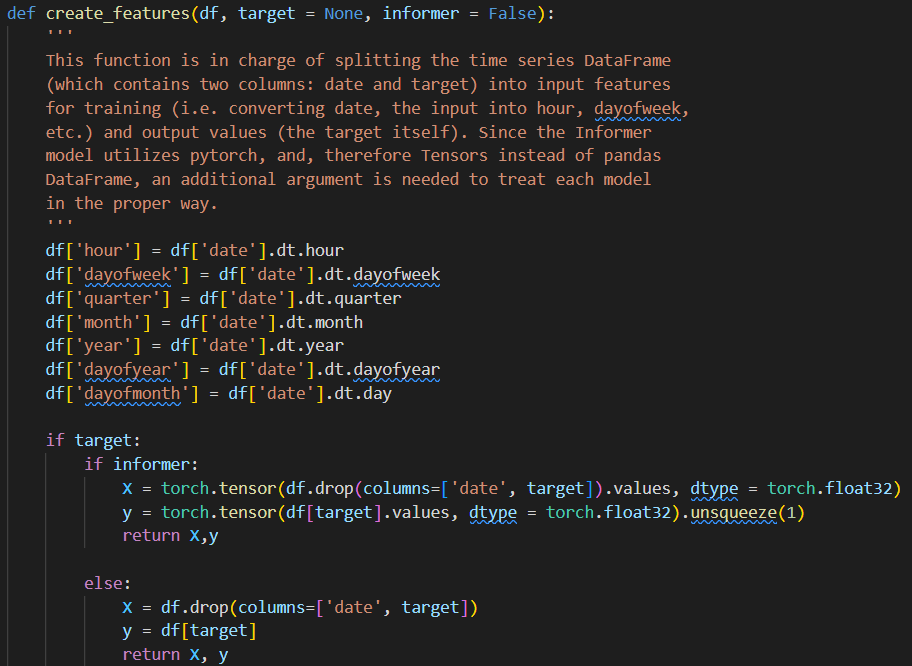
\includegraphics[scale = 0.65]{imgs/ej_module.png}
    \caption{Ejemplo abstracción código con tfg\_module.}
    \label{ejAbstraccion}
\end{figure}

Para emplear los respectivos archivos \Code{.py} de este módulo en los archivos \Code{.py} de los algoritmos, basta con poner las líneas de código mostradas en la Figura \ref{importacionModulo}:

\begin{figure}[H]
    \centering
    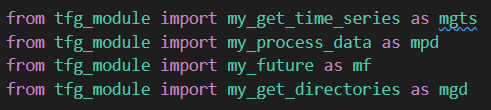
\includegraphics[scale = 0.7]{imgs/importacion_modulo.png}
    \caption[Importación tfg\_module.]{Importación tfg\_module\protect\fnm.}
    \label{importacionModulo}
\end{figure}


\fnt{Para poder importar el módulo, la ubicación de este y de los archivos \Code{.py} debe ser correcta. Véase el repositorio de Github para ver la estructura de carpetas.}


\subsection{Procesamiento de los datos: Creación de modelos}
Una vez los datos están preprocesados debidamente, se puede empezar a procesar estos para poder ser entrenados. La diferencia entre preprocesar los datos y procesarlos radica en que en el primero se transforman los datos en "crudo" en nuevos datos a partir de los existentes, y se extraen las características necesarias para poder entrenar los modelos. El procesamiento de los datos es el paso siguiente en el que,  una vez se tienen los datos para ser entrenados, hay que decidir cómo entrenarlos.

El módulo explicado en el apartado anterior también se encarga, en cierta parte, de procesar los datos. Esto se lleva a cabo en \Code{my\_process\_data.py}. Este archivo cumple con dos funciones principales: crear las características de \ti{input} y \ti{output} para el entrenamiento y testeo de  los algoritmos ---como se vio en la Figura \ref{ejAbstraccion}---. También se encarga de la división de datos en entrenamiento, validación y testeo para el algoritmo de TCN, pues este usa la técnica de evaluación \ti{train-test-split} como se comentará más en profundidad posteriormente en este mismo apartado.

Una vez ya están los datos preprocesados y procesados, se puede empezar a entrenar los algoritmos y generar los respectivos modelos. Todo este proceso se lleva a cabo en la siguiente sección de la arquitectura: véase la Figura \ref{procesamiento}.

\begin{figure}[H]
    \centering
    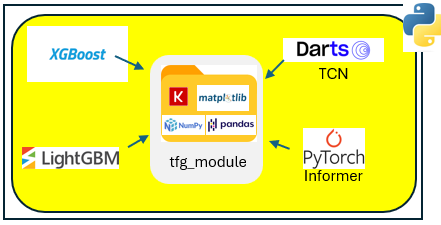
\includegraphics[scale = 0.84]{imgs/procesamiento_datos.png}
    \caption{Procesamiento de los datos y creación de los modelos.}
    \label{procesamiento}
\end{figure}

\subsubsection{Creación de modelos}
Los cuatro algoritmos se han entrenado con los mismos datos. Estos datos de entrenamiento son el archivo \Code{diario.csv} (véase Figura \ref{arquitectura}) con su respectivo preprocesamiento. El objetivo de la predicción será estimar las futuras compras y ventas de la empresa a partir de los datos contables. Pese a que el método de optimización de hiperparámetros para los cuatro algoritmos ha sido el mismo (GridSearch) el procesamiento de los datos ha sido algo distinto para el algoritmo TCN que para el resto. 

\subsubsubsection{Técnicas de evaluación}
Existen enfoques distintos a la hora dividir los datos para poder entrenarlos. 
A esto se le conoce como técnicas de evaluación. El enfoque más común, por su sencillez de aplicación y su rapidez de ejecución, es la división en \ti{train}-\ti{test} \ti{split}. Esto consiste en dividir los datos en un conjunto de entrenamiento (i.e. entrenamiento + validación) y otro conjunto de testeo para, posteriormente, poder evaluar el modelo. Esta es la manera en la que se ha entrenado el algoritmo TCN. Véase la Figura \ref{trainTestSplit}.

\begin{figure}[H]
    \centering
    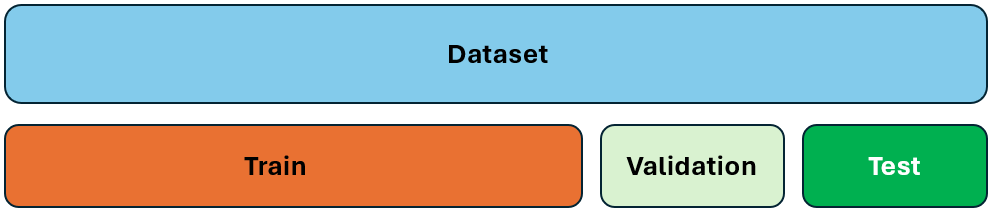
\includegraphics[scale = 0.4]{imgs/trainTestSplit.png}
    \caption{División entrenamiento TCN.}
    \label{trainTestSplit}
\end{figure}

Por otra parte, los algoritmos de XGBoost, LightGBM e Informer han sido entrenados utilizando \ti{K-fold Cross-Validation} (CV). Esta técnica de evaluación es más robusta que la anterior, pero computacionalmente más costosa. La ventaja de CV respecto a la anterior, es que todos los datos son parte del conjunto de entrenamiento y de testeo en algún punto del entrenamiento. Véase la Figura \ref{CV}.

\begin{figure}[H]
    \centering
    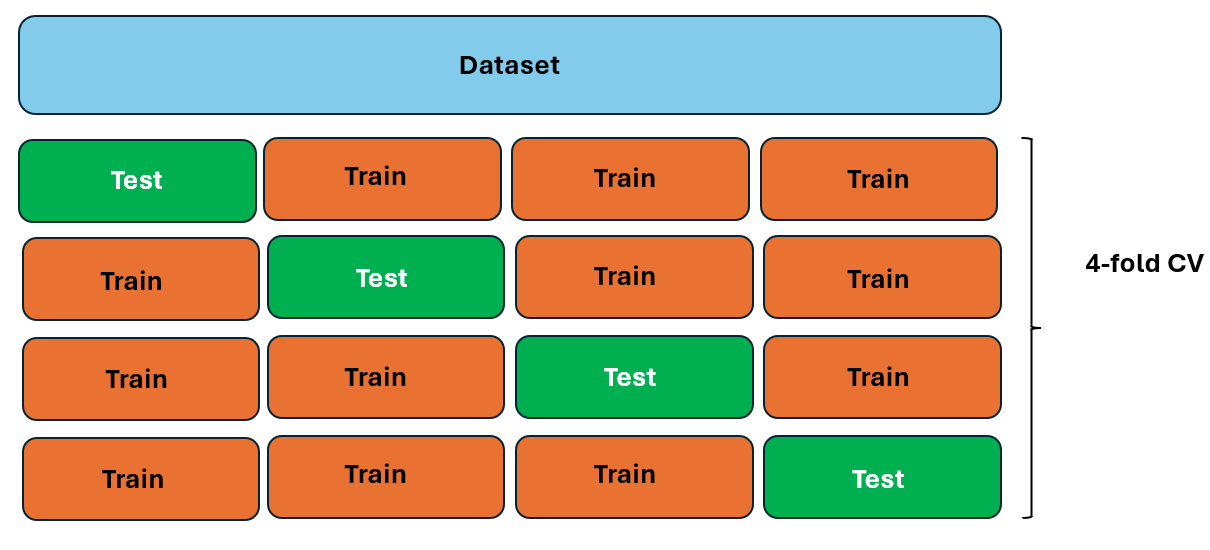
\includegraphics[scale = 0.4]{imgs/cv.png}
    \caption{División entrenamiento XGBoost, LightGBM e Informer.}
    \label{CV}
\end{figure}

Cabe mencionar que el archivo \Code{diario.csv} supone entrenamiento y validación en \ti{train-test split}, mientras que en CV, es el \ti{dataset} entero de la Figura \ref{CV}.

Por último, es importante a recalcar que el uso de distintas técnicas de evaluación para distintos algoritmos es debido a cómo están implementadas las librerías de estos algoritmos.

\subsubsubsection{Optimización de hiperparámetros}
Para encontrar la mejor combinación de hiperparámetros posibles, se ha optado por utilizar el algoritmo de GridSearch. Este algoritmo es computacionalmente muy costoso pero muy eficaz a la hora de encontrar el mejor modelo posible. Recibe un conjunto de posibles valores que se desea 
probar para cada hiperparámetro (e.g. \ti{learning rate}, número de épocas y otros específicos de cada algoritmo de aprendizaje automático). GridSearch lo que realizará es un entrenamiento para cada posible combinación de valores de hiperparámetros y devolverá la combinación de estos que mejor resultado ha obtenido en base a una métrica de monitorización. 

Para el caso de series temporales, se ha optado por utilizar dos métricas de monitorización típicas de este problema de aprendizaje supervisado: \ti{Mean Absolute Error} (MAE) y \ti{Root Mean Squared Error} (RMSE). De esta manera, por cada vez que se entrene un algoritmo, se guardarán dos  modelos: el modelo que mejor métrica MAE haya obtenido; así como el modelo con mejor métrica RMSE. Estos modelos no tienen por qué ser los mismos. De esto se hablará más en profundidad a continuación.

\subsubsubsection{Obtención de mejores resultados}
Una vez el algoritmo se ha entrenado, GridSearch devolverá el mejor modelo encontrado, con sus respectivos parámetros, en base a la métrica (o métricas) estipuladas. Puesto que se aplicarán metodologías MLOps (véase apartado siguiente), se guarda el modelo con su respectiva información relevante. Esta información es:
\begin{itemize}
    \item El mejor modelo para cada métrica.
    \item Parámetros del modelo.
    \item Métrica MAE y RMSE del modelo (tanto para el modelo con mejor MAE, como para el modelo con mejor RMSE).
    \item Un \Code{.csv} con las predicciones del modelo (próximos doce meses, aunque únicamente se utilizarán tres).
    \item Un \Code{.png} con las predicciones realizadas por del modelo.
\end{itemize}

Para este trabajo, esta es la información que se ha considerado relevante almacenar para cada modelo. No obstante, no quiere decir que otro tipo de información adicional no fuera posible. Esta información de cada modelo quedará registrada en la nube, pero esto se comenta más en detalle en el siguiente apartado.

\subsection{MLOps: monitorización y automatización del proceso}
Como se ha mencionado en secciones anteriores, MLOps supone un conjunto de prácticas en el ámbito de aprendizaje automático que permite tener un control y seguimiento del ciclo de vida de los modelos. Todo esto, a ser posible, de  manera automatizada. De esta manera, se consigue tener a disposición siempre el mejor modelo generado hasta el momento. También se facilita la labor de poder comparar modelos generados en un futuro con los modelos actuales para poder ir actualizándolos de manera correcta. Esto es una de las esencias del ciclo de vida de \ti{machine learning}.

\subsubsection{Monitorización de los modelos}
Tener un control del ciclo de vida de los modelos es esencial para tener un versionado correcto e información acerca de ellos más allá del propio modelo. De esta tarea se va a encargar principalmente Mlflow. 

Desplegar un servidor en Mlflow en local es una tarea relativamente sencilla y que se podría haber llevado a cabo en el desarrollo de este trabajo ---pues no es un entorno colaborativo---. De todas maneras, con el objetivo de enfocar este trabajo lo más similar posible a un \B{entorno colaborativo real}, se ha optado por alojar el servidor de Mlflow en Dagshub. Véase la Figura \ref{MLOps} para situar estas tecnologías en la arquitectura de la Figura \ref{arquitectura}.

\begin{figure}[H]
    \centering
    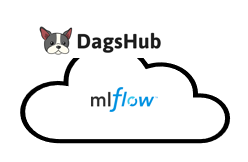
\includegraphics[scale = 0.95]{imgs/MLOps.png}
    \caption{Mlflow alojado en Dagshub.}
    \label{MLOps}
\end{figure}

El único motivo de haber utilizado Dagshub, como se ha dicho, es el de poder tener un servidor de Mlflow en la nube, simulando un entorno colaborativo real. Dagshub, a un nivel alto de abstracción, se puede ver como una extensión de Github pensada para alojar código de inteligencia artificial. De hecho, una de las maneras de iniciar un repositorio en Dagshub es vinculándolo con el repositorio de Github, como se ha hecho en este trabajo. Véase la Figura \ref{dagshubInit}.

\begin{figure}[H]
    \centering
    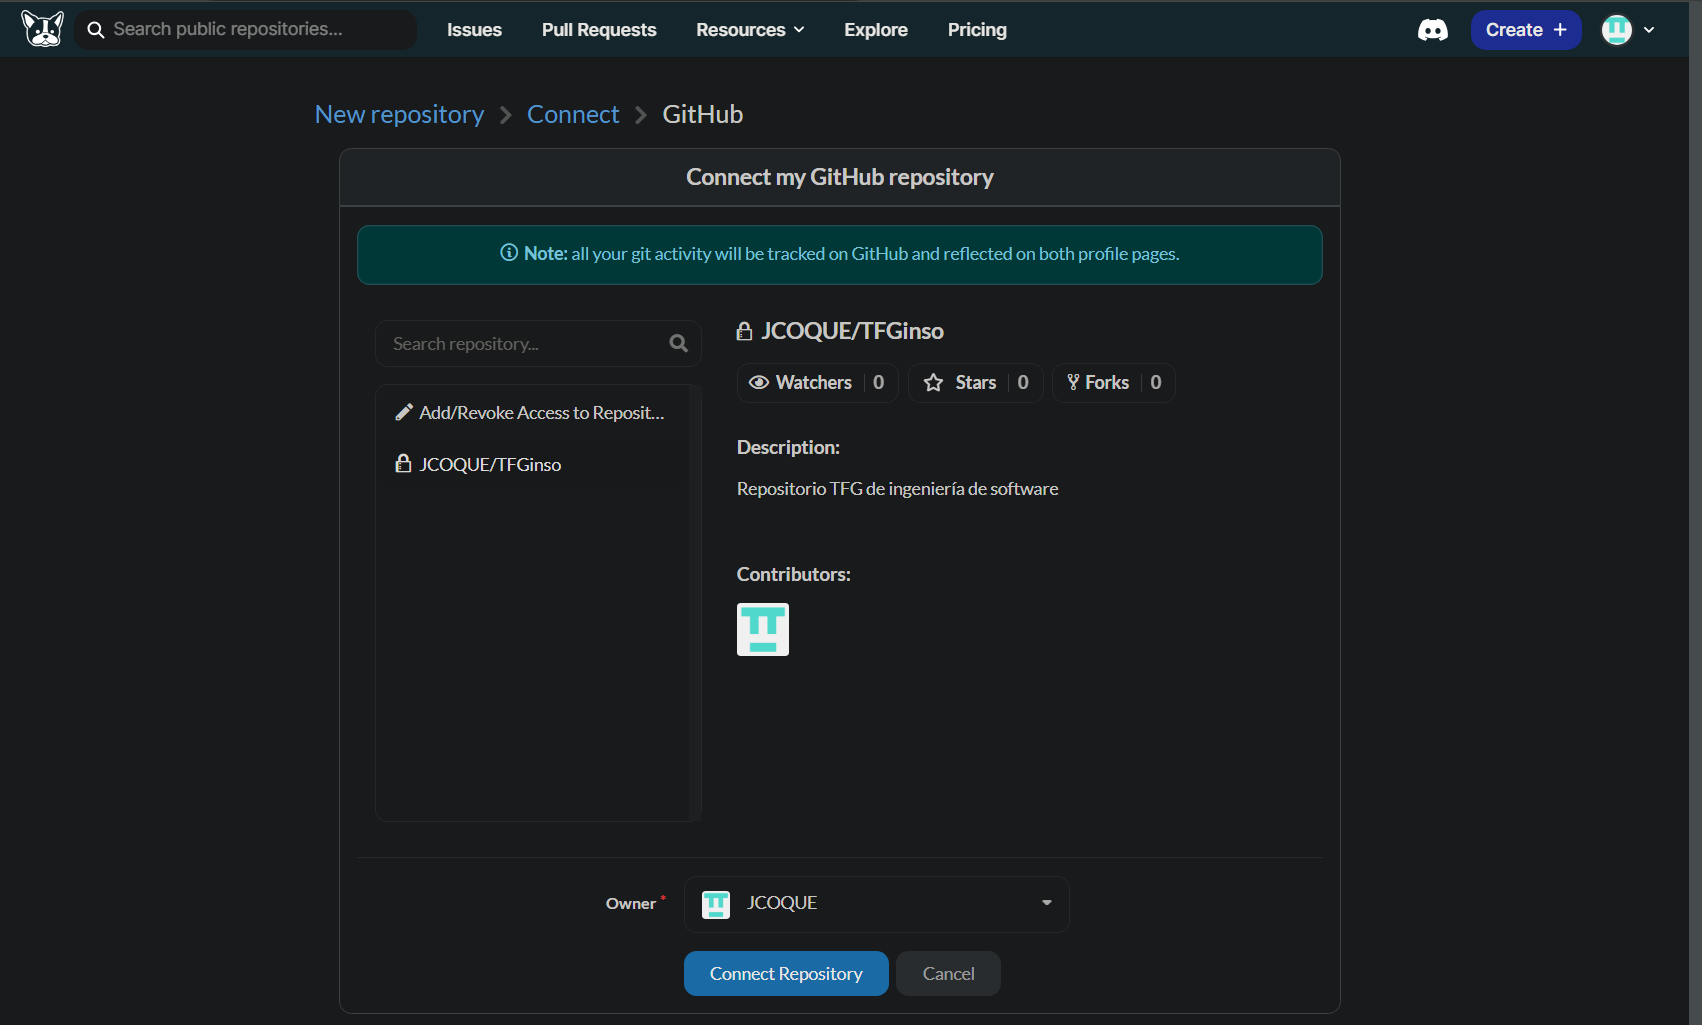
\includegraphics[scale = 0.4]{imgs/dagshub.png}
    \caption[Proceso de vinculación entre el repositorio de Github con  el Dagshub.]{Proceso de vinculación entre el repositorio de Github con  el Dagshub\protect\fnm.}
    \label{dagshubInit}
\end{figure}


\fnt{Aunque en la Figura \ref{dagshubInit} aparezca el nombre de \B{TFGinso} como el nombre del repositorio de Github, este nombre de repositorio se cambió posteriormente a \B{TFG-ingenieria}. Este último es el nombre del repositorio actual en Github.}

Por temas de seguridad, mientras que el repositorio de Github es público, el de Dagshub es privado. De nuevo, simulando un entorno colaborativo real en el que se deja el código de proyecto abierto en Github para poder recibir sugerencias de mejora en el código por parte de gente externa (\ti{pull-requests}), mientras que el versionado de modelos se maneja de manera privada.



Una vez hecho el paso de vincular el repositorio de Github en Dagshub, uno puede ir al botón verde \B{Remote} donde allí encontrará la información  necesaria para poder conectarse tanto al repositorio de Dagshub desde código, como al servidor de Mlflow. Esto se puede ver de manera más visual en la Figura \ref{DasghubConnect}, donde, además, también se puede ver un pequeño ejemplo de cómo iniciar Mlflow y de cómo se guardan los parámetros y métricas de un modelo.

\begin{figure}[H]
    \centering
    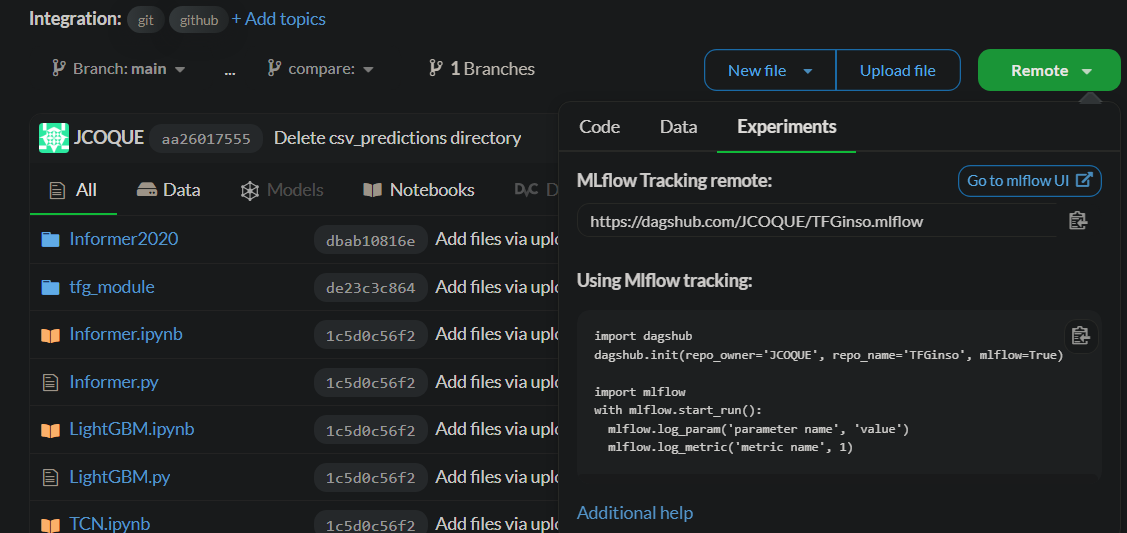
\includegraphics[scale = 0.6]{imgs/dagshub2.png}
    \caption[Comandos para  conectarse a Dagshub y alojar modelos en Mlflow]{Comandos para  conectarse a Dagshub y alojar modelos en Mlflow\protect\fnm.}
    \label{DasghubConnect}
\end{figure}

\fnt{Este repositorio será eliminado al entregar el trabajo, por lo que la información proporcionada en la Figura \ref{DasghubConnect} no será útil.}

En la sección de \ti{Expermients}, tras pulsar el botón verde de \B{Remote}, uno puede ver la sección de:

\begin{itemize}
	\item \B{Mlflow Tracking remote}: url necesaria para conectarse al servidor de Mlflow desde código.
	\item \B{Using Mlflow tracking}: comandos necesarios para inicializar el repositorio de Dagshub desde código Python.
\end{itemize}


En el caso particular de este trabajo, por cada entrenamiento de cada algoritmo, se han almacenado en Mlflow dos modelos: el modelo con mejor métrica de MAE y el modelo con mejor métrica de RMSE ---como se ha comentado con anterioridad---. Adicionalmente a los modelos en sí, se han almacenado:
\begin{itemize}
	\item Parámetros de cada modelo.
	\item Métricas de cada modelo.
	\item Esquema de características de entrenamiento (\ti{inputs}) de cada modelo.
	\item Esqeuma de características de salida (\ti{outputs}) de cada modelo.
	\item Gráfica con las predicciones a doce meses de cada modelo.
	\item \Code{.csv} con las predicciones y su respectiva fecha.
\end{itemize}

Toda esta información irá a parar a lo que Mlflow denomina como ``Experimentos". Por  lo general, un Experimento representa un conjunto de modelos entrenados y almacenados de un algoritmo en concreto. En este trabajo, al tener cuatro algoritmos y dos series temporales (una para Compras y otra para Ventas) se tienen un total de ocho Experimentos. 

Una vez en el código se haya guardado la información pertinente de cada modelo, uno se puede ir a la interfaz gráfica de Mlflow (en el botón azul \ti{Go to Mlflow UI} de la Figura \ref{DasghubConnect}), y visualizar allí sus respectivos experimentos. Además, Mlflow permite comparar distintos modelos (comúnmente de un mismo Experimento, pero se pueden hacer de múltiples) de una manera sencilla. Véase la Figura \ref{mlflowCompare} donde se muestran dos modelos del Experimento ``Compras LightGBM", donde por cada modelo, aparece su esquema de datos de entrada (\ti{Dataset}), métricas, \ti{tags} y otra información relevante.

\begin{figure}[H]
    \centering
    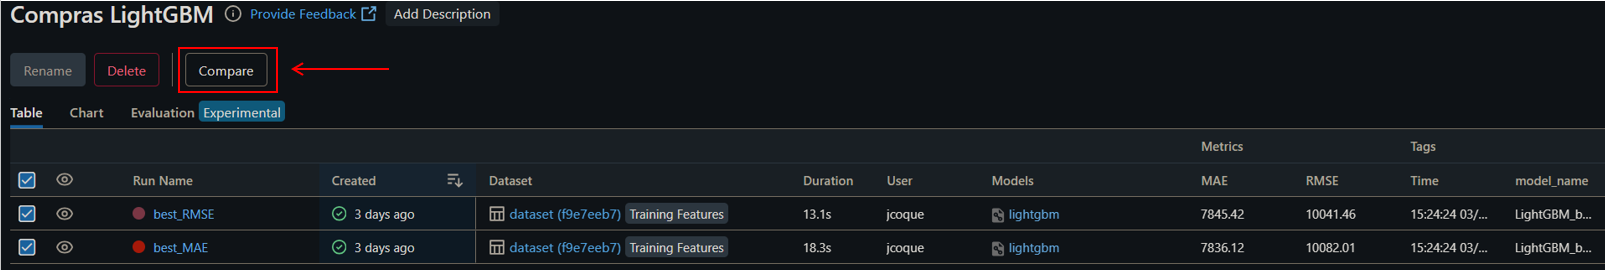
\includegraphics[width = 0.9\textwidth, height= 3.5cm]{imgs/mlflow_compare.png}
    \caption{Ejemplo de modelos almacenados (best\_MAE y  best\_RMSE) para el Experimento ``Compras LightGBM".}
    \label{mlflowCompare}
\end{figure}

Dentro de cada modelo, se puede encontrar información adicional acerca de este. Véase la Figura \ref{MlflowInfo}.

\begin{figure}[H]
    \centering
    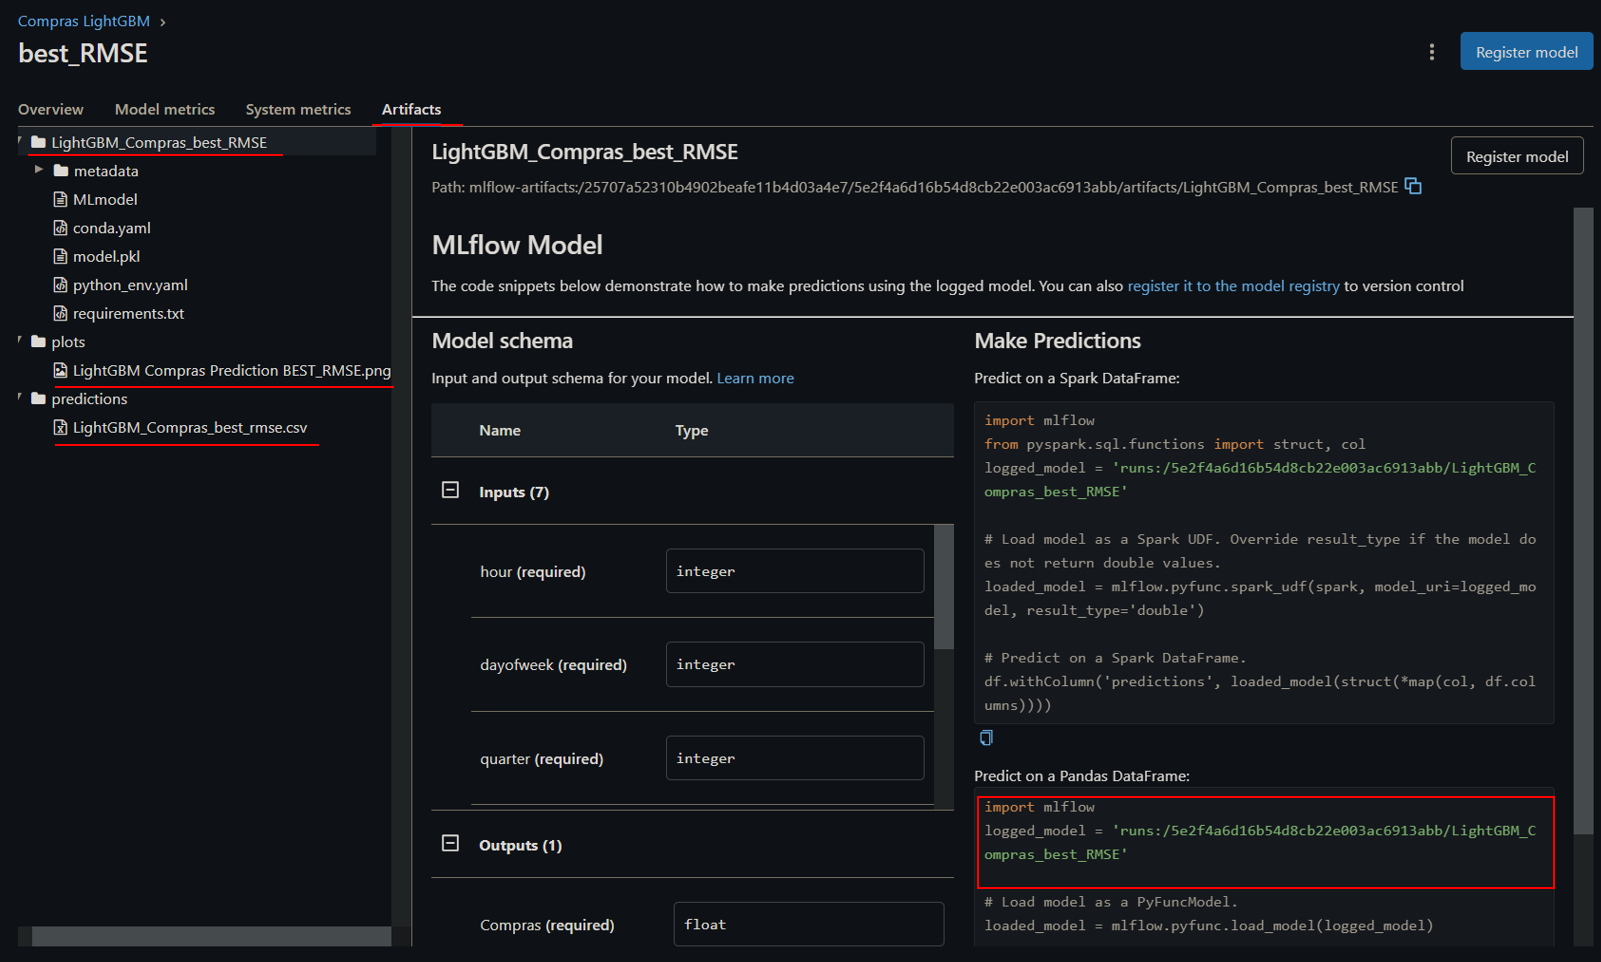
\includegraphics[scale = 0.4]{imgs/mlflow_info.png}
    \caption{Modelo almacenado en Mlflow, junto con la gráfica, datos de predicciones y el respectivo link para recuperarlo.}
    \label{MlflowInfo}
\end{figure}

En la Figura \ref{MlflowInfo}, se puede ver subrayada una sección de Artefactos. Esta sección es común a todos los modelos. En ella se encuentra el modelo almacenado y cómo recuperarlo (cuadrado en rojo de abajo a la derecha). Además, también aparece subrayado la imagen \Code{.png} de las predicciones y el \Code{.csv} con las predicciones en valores numéricos junto con sus respectivas fechas. Por último, en el centro de la imagen, aparece en \B{Model schema} donde se pueden ver las características de entrada (\ti{inputs}) que está recibiendo el modelo, así como las características de salida \ti{output} de este mismo modelo.

Como se dijo al principio de este apartado, todo este proceso de seguimiento y monitorización del ciclo de vida de los modelos de MLOps es conveniente implementarlo y es lo que se haría en un entorno real. Pero además, se busca que todo este proceso explicado hasta ahora, desde el preprocesamiento de los datos hasta la generación y almacenamiento de los modelos, sea de manera \B{automatizada}. Esto se explica en el siguiente apartado.

\subsubsection{Automatización del proceso}
Tener el proceso descrito hasta ahora, desde el preprocesamiento de los datos hasta el almacenamiento de los modelos en Mlflow, de manera automatizada no solo ahorra tiempo, sino que también posibles errores humanos. La contraparte de tener un proceso automatizado, es que se pierde cierto control en el flujo si no se utiliza una herramienta adecuada. Prefect, es la herramienta perfecta para esto, pues ofrece automatización, pero también un seguimiento del flujo de tareas de manera sencilla e intuitiva. Véase la Figura \ref{Prefect} para poder posicionar a Prefect en la arquitectura.

\begin{figure}[H]
    \centering
    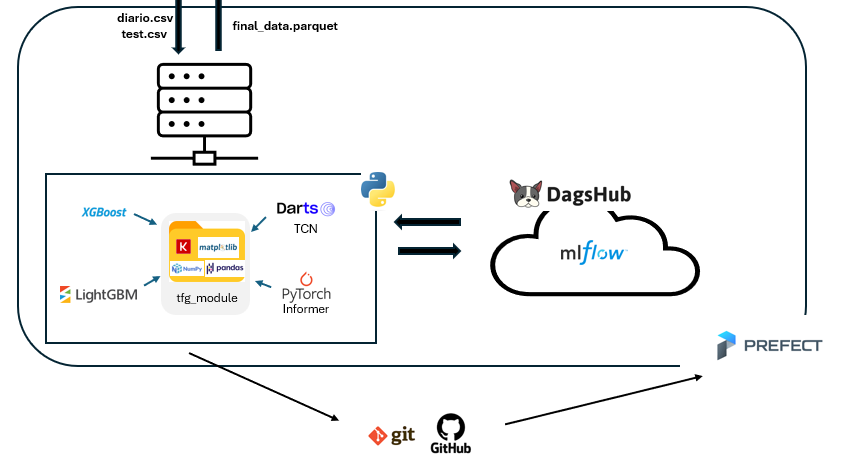
\includegraphics[width = 0.8\textwidth]{imgs/prefect.png}
    \caption{Prefect en la arquitectura del proyecto.}
    \label{Prefect}
\end{figure}

La Figura \ref{Prefect} trata de representar cómo todos los pasos explicados hasta ahora en esta sección los engloba Prefect. Es decir, que están automatizados por esta herramienta. Además, el código que ejecuta Prefect no lo extrae de manera local, sino del repositorio de Github. De nuevo, tratando de simular un entorno colaborativo real.

Para poder continuar, hay que entender algunos conceptos fundamentales de Prefect:
\begin{itemize}
    \item \B{flow}: El código que se ejecuta.
    \item \B{task}: Divide el \ti{flow} en trozos más pequeños para tener un seguimiento mejor de la ejecución.
    \item \B{deployment}: Proceso que permite ejecutar el código de manera automatizada y desde una localización remota (e.g. repositorio Github, como es el caso de este trabajo).
    \item \B{work pool}: Instancia donde se almacenan los flows para poder ejecutarlos.
    \item \B{worker}: Proceso encargado de ejecutar los flows (i.e. el código).
\end{itemize}

Respecto al \ti{flow} y \ti{tasks}, Prefect ofrece los decoradores \Code{@flow} y \Code{@task} que deben ser asignados únicamente a funciones (no pueden ser asociados a métodos de clase y, por eso, esta parte del código en los \Code{.py} de los algoritmos es algo redundante, pues se crean funciones llamadas $X$ que llaman a los métodos de clase  de cada algoritmo con nombre $X$.). Véase la Figura \ref{PrefectDecorators} para poder ver estos decoradores en el código y tener una mejor visualización acerca de estos y de cómo están implementan.

\begin{figure}[H]
    \centering
    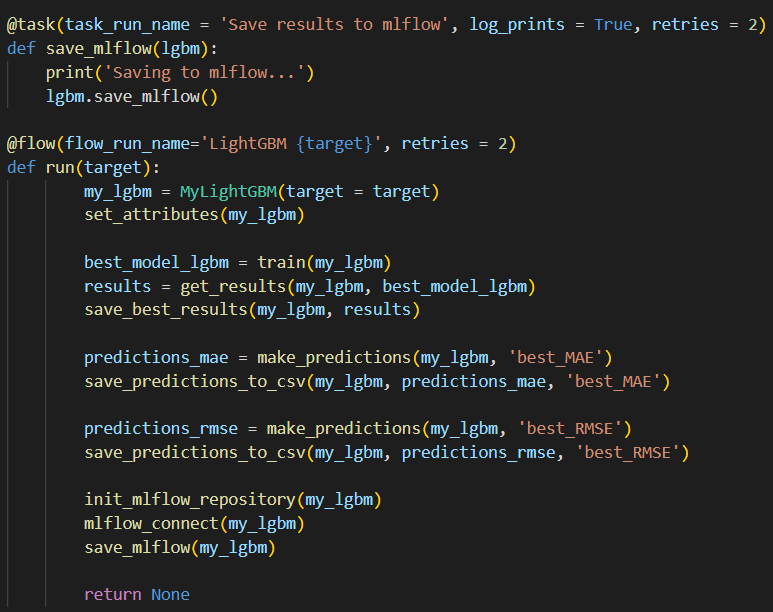
\includegraphics[scale = 0.65]{imgs/prefect_decorators.png}
    \caption{Decoradores de Prefect en el código.}
    \label{PrefectDecorators}
\end{figure}

En la Figura \ref{PrefectDecorators} se puede ver en la función \Code{save\_mlflow()} la redundancia de la que se ha hablado antes. Por el momento Prefect no ha implementado, al menos de manera sencilla, el utilizar sus decoradores en métodos de clase y esta fue la solución que se encontró. Respecto a los decoradores en sí, se puede ver como la función \Code{run()} tiene asociado el decorador \Code{@flow}. Esta función se encarga de llamar a otras funciones, cada una encargada de una cosa. Estas funciones a las que llama, cada una tiene un decorador \Code{@task} asignado. Además, también se puede apreciar en la Figura \ref{PrefectDecorators} algunos parámetros que se han introducido a estos decoradores, como puede ser el nombre o el número de intentos que Prefect debe realizar en caso de que algo vaya mal en la ejecución del código. También está establecido en estos parámetros que los \ti{prints} se guarden en la ejecución de Prefect.

La ejecución de un \ti{flow} entero se vería de la siguiente manera en la interfaz gráfica de Prefect.


\begin{figure}[H]
	\centering
	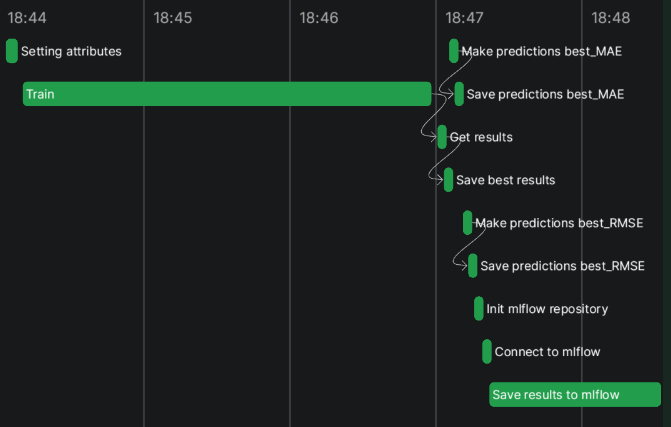
\includegraphics[scale = 0.7]{imgs/prefectUI.png}
	\caption{Flow ejecutado con Prefect.}
	\label{PrefectUI}
\end{figure}

En la Figura \ref{PrefectUI} se puede ver la ejecución de un \ti{flow} entero. Este \ti{flow} está divido en tareas. Si uno se fija bien, las tareas mostradas con la Figura \ref{PrefectUI} son las mismas que las funciones a las que se llama en la función \Code{run()} en la Figura \ref{PrefectDecorators}. También, en la Figura \ref{PrefectUI} se pueden ver algunas flechas que salen de algunas tareas y se dirigen a otras. Esto viene a indicar la \B{dependencia} entre unas tareas y otras. Por ejemplo, hay una flecha que sale de la tarea \ti{Train} y apunta a la tarea \ti{get\_results}, indicando que para ejecutar esta segunda tarea, se debe haber ejecutado la primera antes.

Algo importante a mencionar, y que puede resultar confuso, es que el orden de las tareas está indicado de izquierda a derecha. La altura a  la que está cada tarea en la Figura \ref{PrefectUI} no indica nada.

Por último, la Figura \ref{PrefectUI} viene muy bien parar explicar lo que se ha mencionado al principio de este apartado: Prefect, además de ser una herramienta de automatización, con ella se puede tener un control de la ejecución del código. Y es que, en el caso de la Figura \ref{PrefectUI}, todas las tareas aparecen en verde; indicando que todo  ha ido bien. En caso de que algo hubiera ido mal, se podría saber en qué tarea el código ha fallado. Además de que Prefect proporciona un mensaje de salida con el tipo de error que ha surgido durante la ejecución. Esto para depurar el código es una ventaja y alivio para el programador.


Los otros tres conceptos, \ti{deployment}, \ti{work-pool} y \ti{worker} están muy ligados entre sí. Tienen una relación muy parecida a la que puede tener un sistema pub/sub. Véase la Figura \ref{prefectArq}.

\begin{figure}[H]
    \centering
    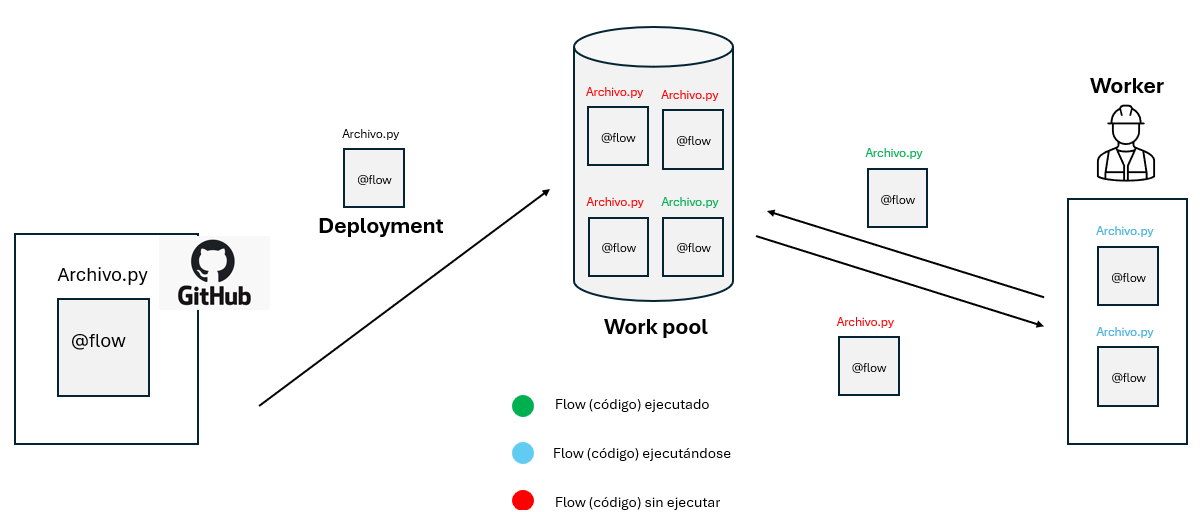
\includegraphics[width = 0.9\textwidth]{imgs/prefect_arquitectura.png}
    \caption{Conceptos deployment, work-pool y worker de manera visual.}
    \label{prefectArq}
\end{figure}

Hasta ahora, se ha explicado cómo funciona la ejecución de un código con Prefect: a través de sus decoradores \Code{@flow} y \Code{@task}. Pero esto no es suficiente para poder automatizar esta ejecución. Para ello está el \ti{deployment}. El \ti{deployment} es una característica de Prefect que lleva el código a ejecutar a un escalón por encima. Esto implica que:
\begin{itemize}
	\item El código se pueda ejecutar de manera automatizada.
	\item Se pueda leer el código a ejecutar desde donde sea; no necesariamente en local. En el caso de este trabajo, el código a ejecutar se extrae de Github. Se quiere dejar esto claro para que se pueda entender mejor la Figura \ref{arquitectura}.
	\item Se pueda ejecutar este código en un entorno que se desee. Idealmente en un servidor con capacidad de entrenar varios modelos al mismo tiempo de manera eficiente. En el caso de este trabajo, se ha utilizado el propio ordenador.
\end{itemize}

Para esto último, es necesario asociar el \ti{deployment} con un \ti{work-pool}. La Figura \ref{prefectArq} trata de representar cómo el \ti{deployment} extrae el código de Github y lo encola en su \ti{work-pool} asociado. En este \ti{work-pool} es donde se aloja el código (los \ti{flows}) que el \ti{worker} descarga, ejecutará y devolverá el resultado de la ejecución. 

Para más información de los comandos empleados para el despliegue de la arquitectura mostrada en la Figura \ref{prefectArq}, están todos explicados en el \href{https://github.com/JCOQUE/TFG-ingenieria/blob/main/README.md}{README.md} de Github en la sección \ti{Commands and other important info to keep in mind.}



\begin{nota}
Aunque no se ha hecho por simplificar contenido de trabajo, se podrían haber duplicado todos los archivos \Code{.py} de los algoritmos y haber configurado los \ti{deployments} para ejecutar, de manera programada, los algoritmos para entrenar la serie temporal de Compras y, por otra parte, para entrenar la serie temporal de Ventas. En caso de que se requiriese, sería muy sencillo implementarlo.
\end{nota}

\subsection{Comparativa de modelos}
En este apartado se explicará la comparativa de modelos. Antes que nada, mencionar que debido a la falta de tiempo, pero sobre todo de recursos, únicamente ha sido posible comparar los algoritmos de LightGBM y TCN. Era de esperar que XGBoost e Informer,  ambos por su complejidad de arquitectura, iban a ser los que más tiempo iban a demandar. Estos algoritmos se tuvieron que dejar de entrenar cuando llevaban más de dos días entrenándose y su consumición de recursos provocaban lentitud en el ordenador, dificultando la realización de otras tareas. En un entorno con una máquina más potente, esto no hubiera supuesto ningún problema.

Para evaluar los modelos, se hace uso del archivo \Code{test.csv}. Esto es para poder comparar datos reales con datos que el modelo no ha visto ---en el entrenamiento---, pero sí ha predicho.

Tanto para Compras como para Ventas se han comparado cuatro modelos en total: 
\begin{itemize}
	\item LightGBM best\_RMSE
    \item LightGBM best\_MAE
    \item TCN best\_RMSE
    \item TCN best\_MAE
\end{itemize}

En ambos casos, Compras y Ventas, TCN ha obtenido un rendimiento mayor, llegando a ajustarse muy bien a los datos de testeo en la serie temporal de Compras. En Ventas, por otra parte, los resultados no han sido tan buenos. 

\subsubsection{Compras}

Véase en la Tabla \ref{comparisonCompras} para poder ver las métricas de los modelos para Compras.

\begin{table}[H]
	\centering
	\begin{tabular}{|c|c|c|}
		\hline
		\multicolumn{3}{|c|}{\textbf{Compras}} \\ \hline
		\multirow{2}{*}{\B{LightGBM best\_RMSE}} & \B{RMSE} & 10041.46 \\ \cline{2-3}
		& \B{MAE} & \cellcolor{red!10}7845.42 \\ \hline
		\multirow{2}{*}{\B{LightGBM best\_MAE}} & \B{RMSE} & \cellcolor{red!10}10082.01 \\ \cline{2-3}
		& \B{MAE} & 7836.12 \\ \hline
		\multirow{2}{*}{\B{TCN best\_RMSE}} & \B{RMSE} & \cellcolor{green!10}6317.86 \\ \cline{2-3}
		& \B{MAE} & 6756.17 \\ \hline
		\multirow{2}{*}{\B{TCN best\_MAE}} & \B{RMSE} & 7589.41 \\ \cline{2-3}
		& \B{MAE} & \cellcolor{green!10}4976.97 \\ \hline
	\end{tabular}
	\caption{Comparativa de métricas entre distintos modelos para Compras.}
	\label{comparisonCompras}
\end{table}

Las métricas, tanto de RMSE como de MAE, no indican si un modelo es bueno o no. Es decir, un MAE de 0.01, por ejemplo, puede ser mucho o poco dependiendo de los datos del problema. Lo mismo ocurre RMSE. Sin embargo, estas métricas sí que sirven para poder determinar, \ti{a priori}, si un modelo es mejor que otro. Estas métricas, al contrario que ocurre con otras muchas, se trata de buscar que su valor sea lo mínimo posible. Con esto mencionado, a partir de los datos mostrados en la Tabla \ref{comparisonCompras}, a primera vista se puede ver que los modelos generados por este algoritmo TCN parecen mejores que los algoritmos generados por este algoritmo de LightGBM.

Se hace un inciso en que esta comparativa no es definitiva, pues también se deben contrastar los datos reales con los datos predichos en una gráfica. Esto es porque  las series temporales tienen fluctuaciones, tendencias y estacionalidades. Lo que se trata de buscar con las predicciones de un modelo, es que este modelo haya ``aprendido" estas características de la serie temporal dada y lo haya sabido plasmar en sus predicciones. De esta manera, no solo un modelo es mejor que otro si obtiene, en este caso, unas métricas con un valor menor, sino también si ha sido capaz de aprender de una manera más eficaz estas propiedades mencionadas recientemente de la serie temporal.
Véase la Figura \ref{comparativaCompras} para ver de manera gráfica los datos de testeo (reales) con las predicciones realizadas por cada modelo.

\begin{figure}[H]
	\centering
	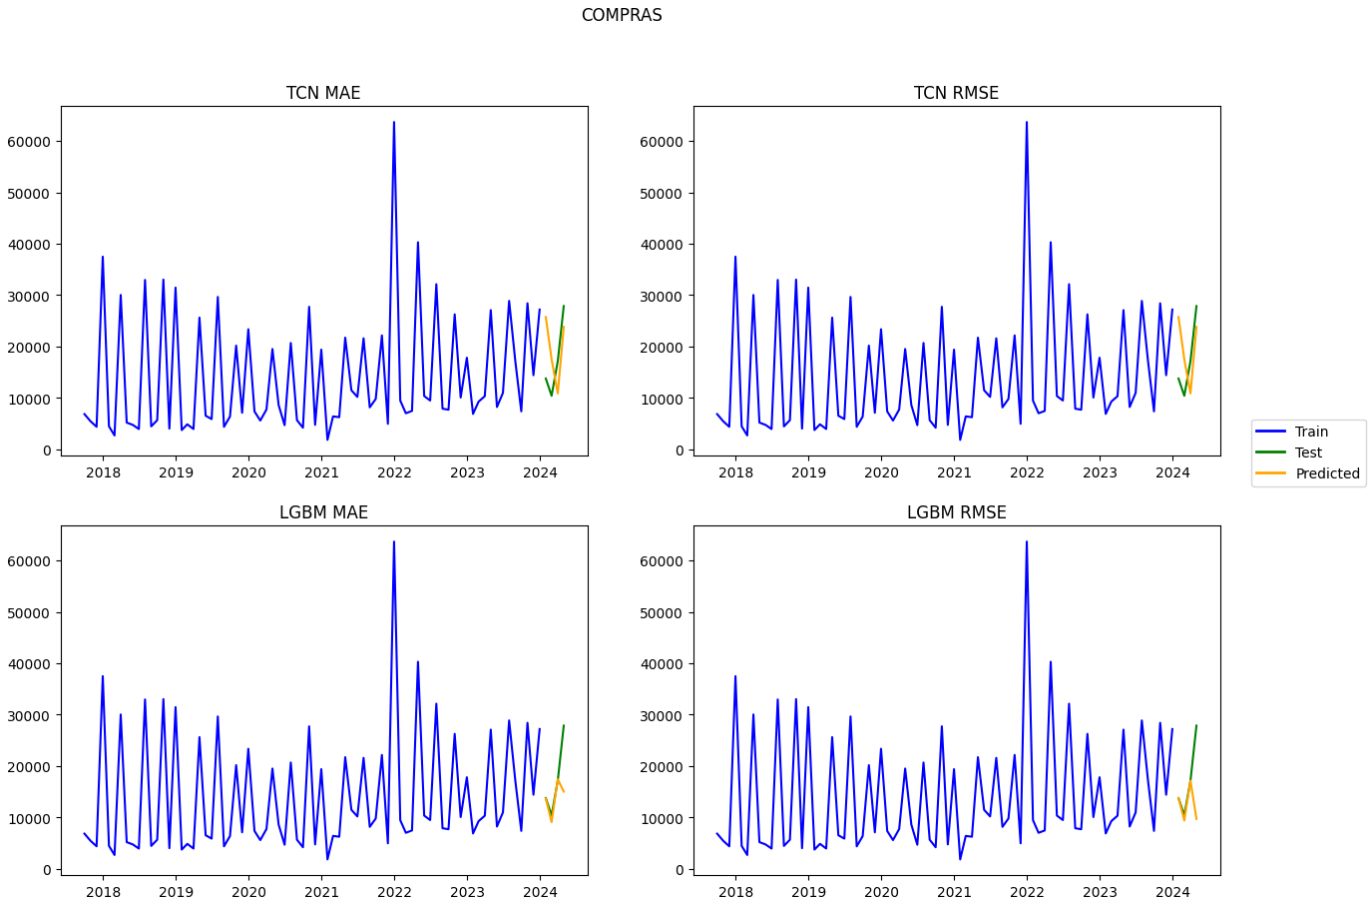
\includegraphics[scale = 0.5]{imgs/comparativaCompras}
	\caption{Datos de testeo junto con las predicciones de cada modelo de Compras visualizado de una manera gráfica.}
	\label{comparativaCompras}
\end{figure}

En la Figura \ref{comparativaCompras} se puede ver de manera mucho más clara que TCN, \B{en este caso}, predice mejor que el algoritmo LightGBM. No solo obtiene mejores métricas ---como se vio en la Tabla \ref{comparisonCompras}---, sino que también se ajusta de manera mucho más precisa a los datos de testeo. Además, es interesante ver cómo, para la serie temporal de compras, TCN ha aprendido muy bien los patrones y tendencias de la serie temporal. Las fluctuaciones las ajusta muy bien.

También cabe mencionar que, al ser las series temporales la consecuencia de un proceso estocástico, más modelos deberían generarse, con sus respectivas comparativas para poder afirmar que el algoritmo TCN es superior a LightGBM en este caso. Las conclusiones de la comparativa, por tanto, son que para los modelos generados, el algoritmo TCN se ajusta mejor que el de LightGBM. Una comparativa más exhaustiva suponía un tiempo de computación inviable con los recursos de  los que se disponía.

Debido a que ambos modelos de TCN son muy parecidos (en cuanto a parámetros y métricas obtenidas), las predicciones las realizan de manera muy similar. Se podrían emplear ambos algoritmos para generar una única predicción. En el caso de este trabajo en concreto, se ha optado por elegir al modelo \B{TCN best\_RMSE}, ya que se ajusta ligeramente mejor a los datos de testeo mostrados en la Figura \ref{comparativaCompras}. Las predicciones realizadas por este algoritmo serán las predicciones mostradas  de manera visual en el último apartado de esta sección.

\subsubsection{Ventas}
La misma lógica de comparativa que se ha explicado en Compras, también se aplica para Ventas. De nuevo, se van a mostrar en una tabla las distintas métricas para cada modelo entrenado ---que son los mismos\fnm\ que en el apartado anterior, pero para la serie temporal de Ventas---, así como una gráfica que mostrará los datos de testeo junto con las predicciones realizadas por cada modelo. Para ver las métricas de cada modelo entrenado en este trabajo, véase la Tabla \ref{comparisonVentas}.

\fnt{Los modelos en sí son distintos. Se han entrenado con series temporales distintas. Lo que es igual son los algoritmos obtenidos y el nombre de sus modelos.}

\begin{table}[H]
	\centering
	\begin{tabular}{|c|c|c|}
		\hline
		\multicolumn{3}{|c|}{\textbf{Ventas}} \\ \hline
		\multirow{2}{*}{\B{LightGBM best\_RMSE}} & \B{RMSE} & 4320.92 \\ \cline{2-3}
		& \B{MAE} & \cellcolor{red!10}3442.7 \\ \hline
		\multirow{2}{*}{\B{LightGBM best\_MAE}} & \B{RMSE} & \cellcolor{red!10}4321.27 \\ \cline{2-3}
		& \B{MAE} & 3442.56 \\ \hline
		\multirow{2}{*}{\B{TCN best\_RMSE}} & \B{RMSE} & \cellcolor{green!10}3086.34 \\ \cline{2-3}
		& \B{MAE} & 4354.17 \\ \hline
		\multirow{2}{*}{\B{TCN best\_MAE}} & \B{RMSE} & 3096.51 \\ \cline{2-3}
		& \B{MAE} & \cellcolor{green!10}2407.42 \\ \hline
	\end{tabular}
	\caption{Comparativa de métricas entre distintos modelos para Ventas.}
	\label{comparisonVentas}
\end{table}

De nuevo, el algoritmo de TCN, en una primera instancia, parece haber sido más eficaz a la hora de estimar la variable objetivo: Ventas en este caso. Sin embargo, este ejemplo viene muy bien para recalcar lo que se  ha mencionado en el apartado anterior: MAE y RMSE no son métricas que indiquen si un modelo es bueno o no. En este caso, el  valor de las métricas es más bajo que para la variable objetivo de Compras del apartado anterior. En una primera instancia, uno podría pensar que estos modelos habrán obtenido mejores resultados; pues sus métricas son mucho más bajas. Pero, como se verá a continuación, para nada es así. Véase la Figura \ref{comparativaVentas} para ver gráficamente los datos de testeo junto con las estimaciones realizadas por cada modelo.

\begin{figure}[H]
	\centering
	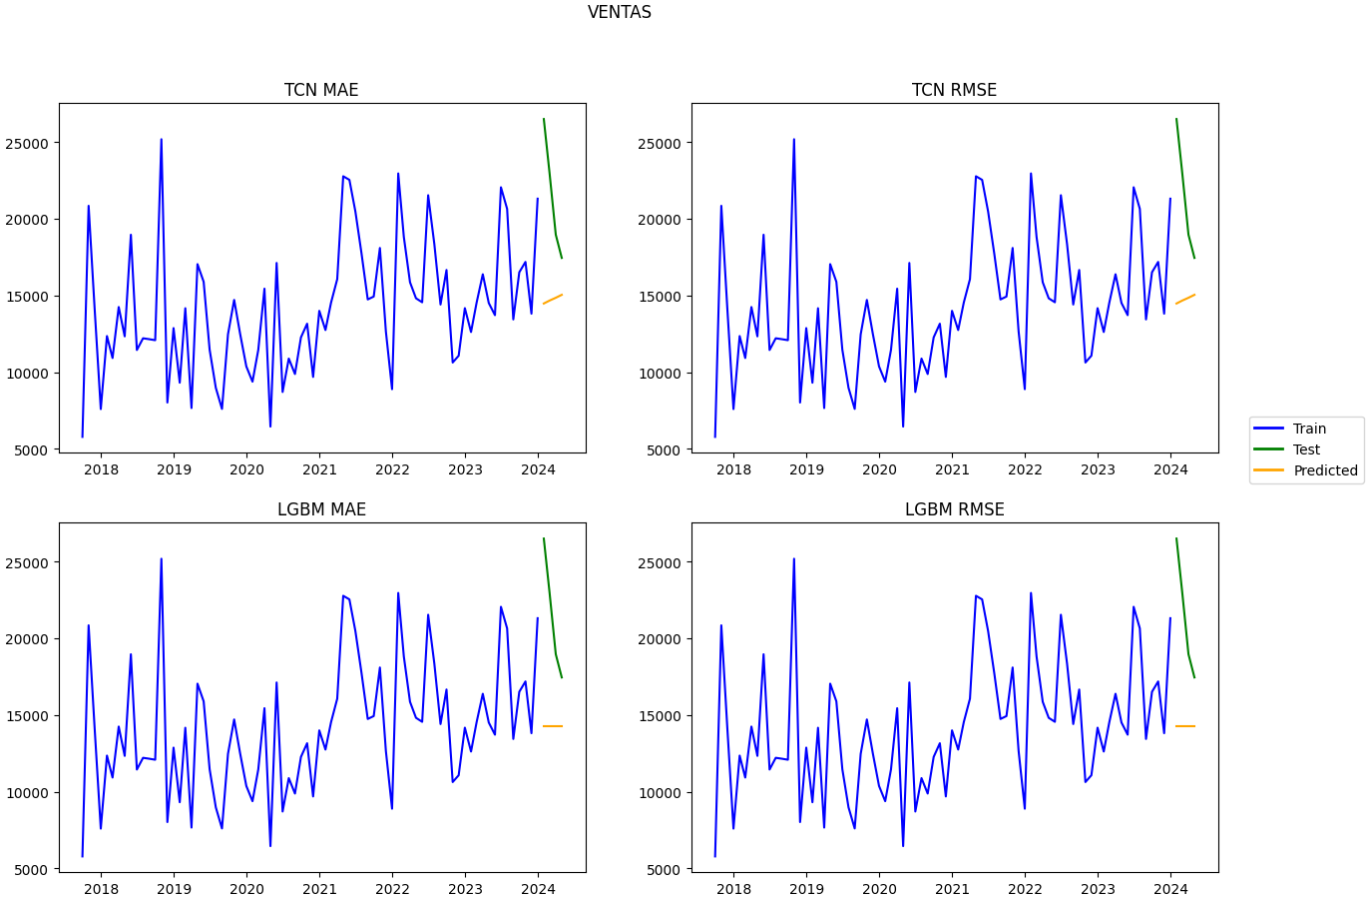
\includegraphics[scale = 0.5]{imgs/comparativaVentas}
	\caption{Datos de testeo junto con las predicciones de cada modelo de Ventas visualizado de una manera gráfica.}
	\label{comparativaVentas}
\end{figure}

En este caso, por lo que muestran las gráficas, ningún algoritmo ha sido capaz de aprender bien las fluctuaciones, tendencias y estacionalidad de la serie temporal. Si uno compara ambas series temporales, esta segunda es mucho más compleja de tratar de predecir: no tiene un patrón tan claro como la serie temporal de Compras. Esto se deba seguramente a cómo se lleva internamente la contabilidad dentro de la empresa y de la manera en que se hacen los cobros y pagos en ella.

Se podrían estudiar los modelos más en profundidad, cómo mejorarlos, tratar de averiguar por qué no han predicho tan bien como en Compras, plantear otros enfoques de entrenamiento como puede ser Optuna, etc. Esto es un trabajo de semanas, y en este trabajo, por falta de tiempo, no se ha cubierto. 

Debido a las métricas obtenidas, se ha elegido el modelo \B{TCN best\_MAE} como modelo candidato a que sus predicciones sean las que aparezcan en las visualizaciones finales.

\subsubsection{Datos finales}
Una vez se han elegido a los modelos candidatos de Compras y Ventas para mostrar sus estimaciones, lo que se hace es juntar toda la información, la presente y la futura, en un \Code{.parquet} que se envía a Azure Blob Storage. Estos datos finales suponen la concatenación de toda la información disponible hasta el momento. Esto es el \Code{diario.csv}, el cual contiene la mayoría de datos. El archivo \Code{test.csv} que tiene el mismo formato y misma estructura que el archivo anterior, pero con datos más actuales. Y, finalmente, después de concatenar estos dos archivos mencionados, se añaden las predicciones de Compras y Ventas de los respectivos modelos elegidos en los apartados anteriores.

Estos  datos concatenados forman el archivo \Code{final\_data.parquet}.  Este archivo supone los datos a almacenar en Azure SQL Database y, por ende, los que utilizará Power BI en sus visualizaciones. El formato \Code{.parquet} se ha elegido por ser un formato que almacena los datos de manera más eficiente y, por tanto, ocupa menos que un \Code{.csv} u otras extensiones; perfecto para entornos de \ti{Big Data}.

\subsection{Almacenamiento de los datos}
En este apartado se explicarán los servicios utilizados en este trabajo para el almacenamiento de los datos. Todo se ha llevado en Azure. De esta manera, los datos están alojados en un lugar seguro y accesible desde cualquier parte del mundo para una persona con los permisos adecuados. De nuevo, al igual que se ha mencionado en apartados anteriores, \B{simulando un entorno real colaborativo}. Véase la Figura \ref{azure}.

\begin{figure}[H]
    \centering
    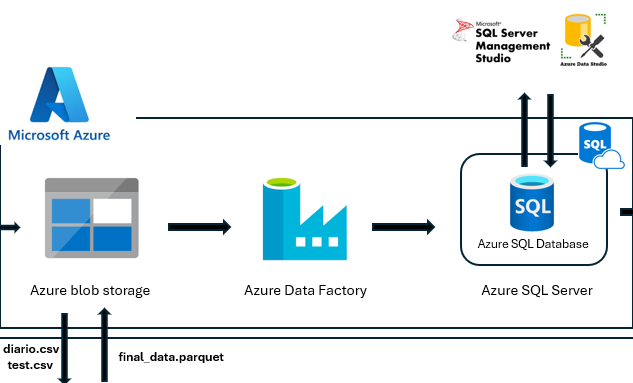
\includegraphics[scale = 0.65]{imgs/azure.png}
    \caption{Arquitectura Azure.}
    \label{azure}
\end{figure}

Aunque no se haya mencionado hasta ahora, todo empieza aquí: en Azure Blob Storage. Se trata de un \ti{datalake} en donde se puede guardar casi cualquier tipo de dato; estructurado, semi-estructurado o no estructurado. Es de este origen de donde el archivo \Code{my\_azure.py}, explicado en el apartado de preprocesamiento, extrae los datos (\ti{pull}) y, asimismo, envía los datos (\ti{push}) una vez estos ya contienen la información necesaria para poder ser visualizados (como se mencionó en el apartado anterior). Véase la Figura \ref{ABS} en donde se muestra una imagen con el contenido de Azure Blob Storage.

\begin{figure}[H]
	\centering
	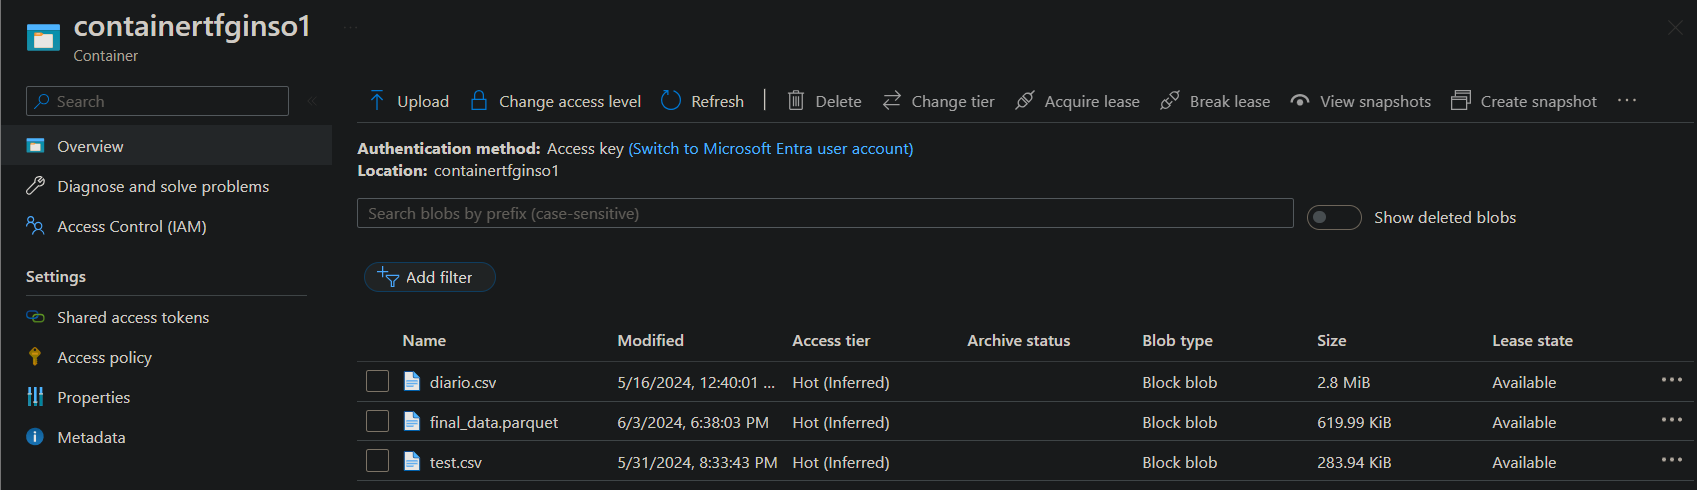
\includegraphics[width = 1\textwidth]{imgs/ABS}
	\caption{Contenido de Azure Blob Storage.}
	\label{ABS}
\end{figure}

Estos archivos se alojan dentro de un contenedor llamado ``containertfginso1" ---como se puede ver arriba a la izquierda de la Figura \ref{ABS}---. Esto es importante tenerlo en cuenta para secciones posteriores, en donde se hará referencia a este contenedor para seleccionar la información que se desea copiar desde Azure Blob Storage a Azure SQL Database (\Code{final\_data.parquet} en este caso).


Ahora, aunque se discutirá más en profundidad en la siguiente sección, por el momento basta con saber que a la aplicación Power BI le conviene que los datos vengan de una base de datos SQL y no de un \ti{datalake}. Esto es porque de esta manera se actualizan los datos de manera más eficiente. Para poder llevar los datos desde Azure Blob Storage en formato \Code{.parquet} a una tabla de base de datos SQL, se  utitliza Azure Data Factory. Este servicio ofrece múltiples \B{actividades} para crear \ti{pipelines} y transportar datos de un origen a un destino. La actividad de interés para este trabajo es \ti{Copy Activity} que se encarga de copiar datos desde Azure Blob Storage hasta Azure SQL Database. Para ello es necesario crear lo que Azure llama \ti{Linked Services} y \ti{Datasets} ---tanto para Azure Blob Storage como para Azure SQL Database---. Por tanto, una arquitectura de Azure que muestre de manera más precisa lo que está ocurriendo es la siguiente; véase la  Figura \ref{azure}:

\begin{figure}[H]
    \centering
    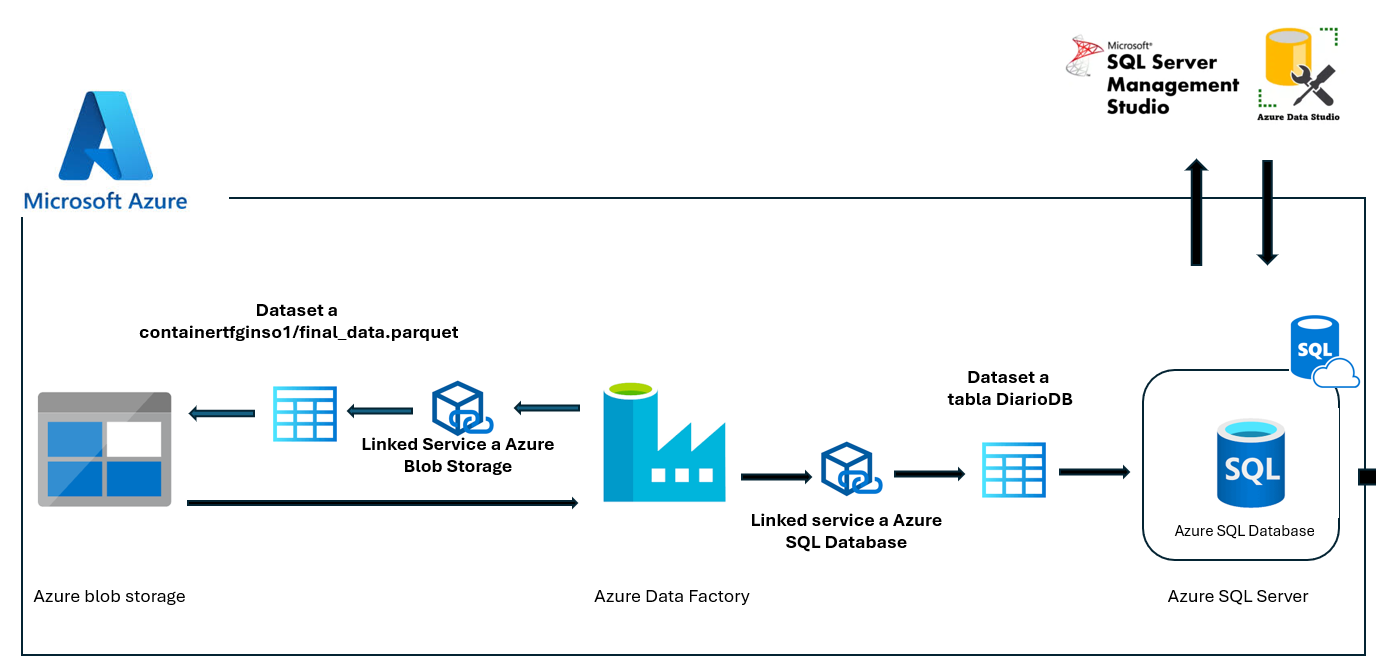
\includegraphics[scale = 0.5]{imgs/azure_arquitecture.png}
    \caption{Arquitectura pura de Azure.}
    \label{realAzure}
\end{figure}

Puesto que Azure Data Factory se puede conectar a varios orígenes de datos, los \ti{Linked Services} le indican a qué origen de datos debe conectarse y cómo hacerlo. En la Figura \ref{realAzure} hay dos \ti{Linked Services} distintos: uno para Azure Blob Storage y otro para Azure SQL Database. 


Una vez hecho este paso, se debe indicar a Azure Data Factory qué datos interesa recopilar del origen y hacia dónde interesa llevarlos en el destino. Para ello están los \ti{Datasets}. El \ti{Dataset} de Azure Blob Storage le indica a Azure Data Factory que debe coger el archivo \Code{containertfginso1/final\_data.parquet} de Azure Blob Storage. Por el contrario, el \ti{Dataset} de Azure SQL Database le indica a Azure Data Factory hacia dónde debe mover estos datos: en este caso a la tabla \Code{diarioDB} de la base de datos SQL creada a través de la herramienta \ti{SQL Server Management Studio}. En la Figura \ref{Datasets} se muestra la configuración de cada uno de los \ti{Datasets} empleados en este trabajo.

\begin{figure}[H]
	\centering
	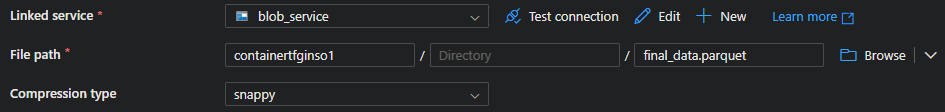
\includegraphics[width = 1\textwidth]{imgs/DatasetAzure}
	\vspace{0.075cm}
	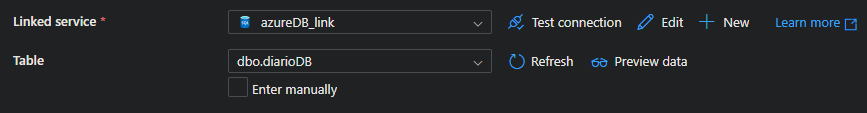
\includegraphics[width = 1\textwidth]{imgs/DatasetAzure2}
	\caption{Configuración \ti{Datasets}.}
	\label{Datasets}
\end{figure}

En la Figura \ref{Datasets} se puede ver cómo cada \ti{Dataset} tiene su propio \ti{Linked Service} asociado. Así como también están especificados los orígenes y destinos de los datos de una manera más concreta.

Dos últimas cosas a tener en cuenta es la configuración de ``mappeo" entre los datos de origen y destino ---cerciorarse de que están bien---. Esto se tuvo que modificar en el trabajo. Véase la Figura \ref{mappeo}.

\begin{figure}[H]
	\centering
		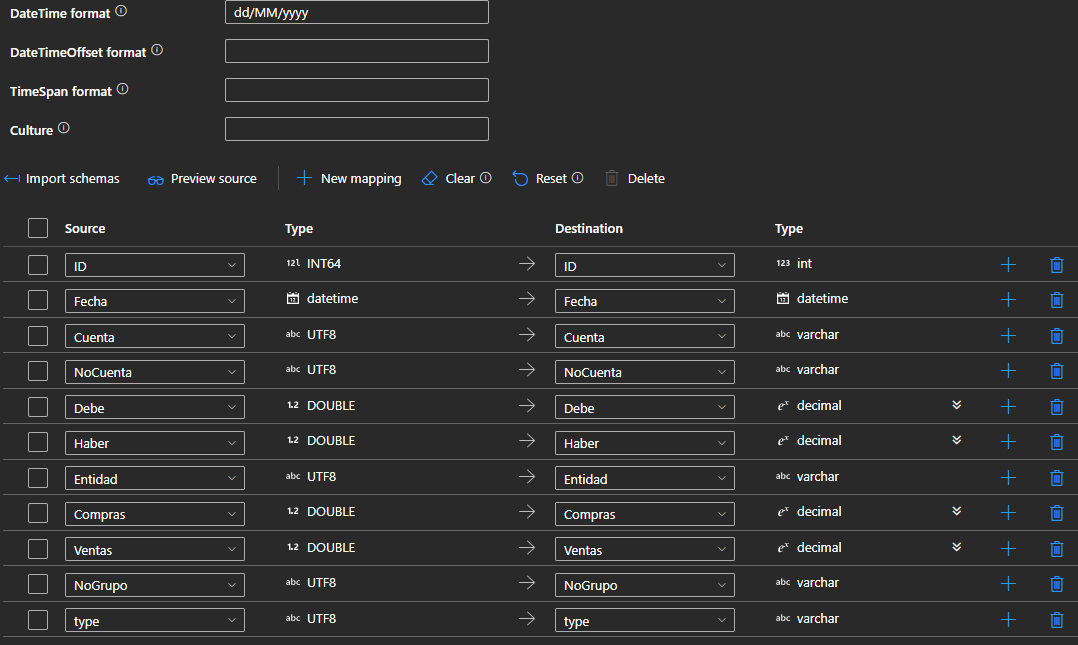
\includegraphics[scale = 0.4]{imgs/dataFactoryconf2.png}
	\caption{Mappeo entre origen y destino.}
	\label{mappeo}
\end{figure}


Por otra parte, la configuración a introducción de datos en la tabla SQL en modo \B{upsert} (\ti{update} + \ti{insert}) ---para solo copiar datos nuevos y/o actualizar los que ya había---. Para determinar si un dato es nuevo (y por tanto debe introducirse) o, por el contrario, ya está en la base de datos (y por tanto debe actualizarse), se le indica a Azure Data Factory que debe fijarse en la columna ID de los datos. De nuevo, esta configuración está pensada para entornos \ti{Big Data} en los que hay una gran cantidad de datos y se trata de optimizar este proceso lo máximo posible. Véase la Figura \ref{dataFactoryconf}.

\begin{figure}[H]
	\centering
	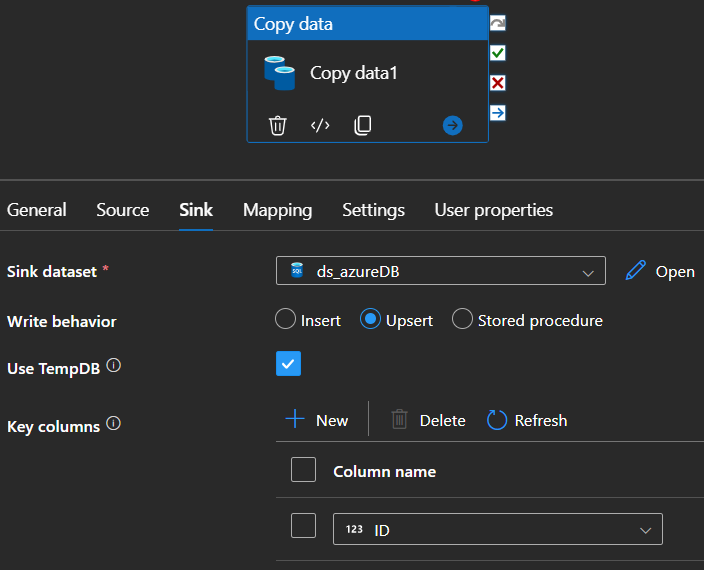
\includegraphics[width = 0.47\textwidth]{imgs/dataFactoryconf1.png}
	\caption{Configuración de upsert con su respectiva columna ID.}
	\label{dataFactoryconf}
\end{figure}

Con todo esto, añadido a la \ti{Copy Activity}, se zure SQL Database. En la Figura \ref{DataFactory} se muestra un esquema con el resultado de realizar esta actividad de copia.

\begin{figure}[H]
    \centering
    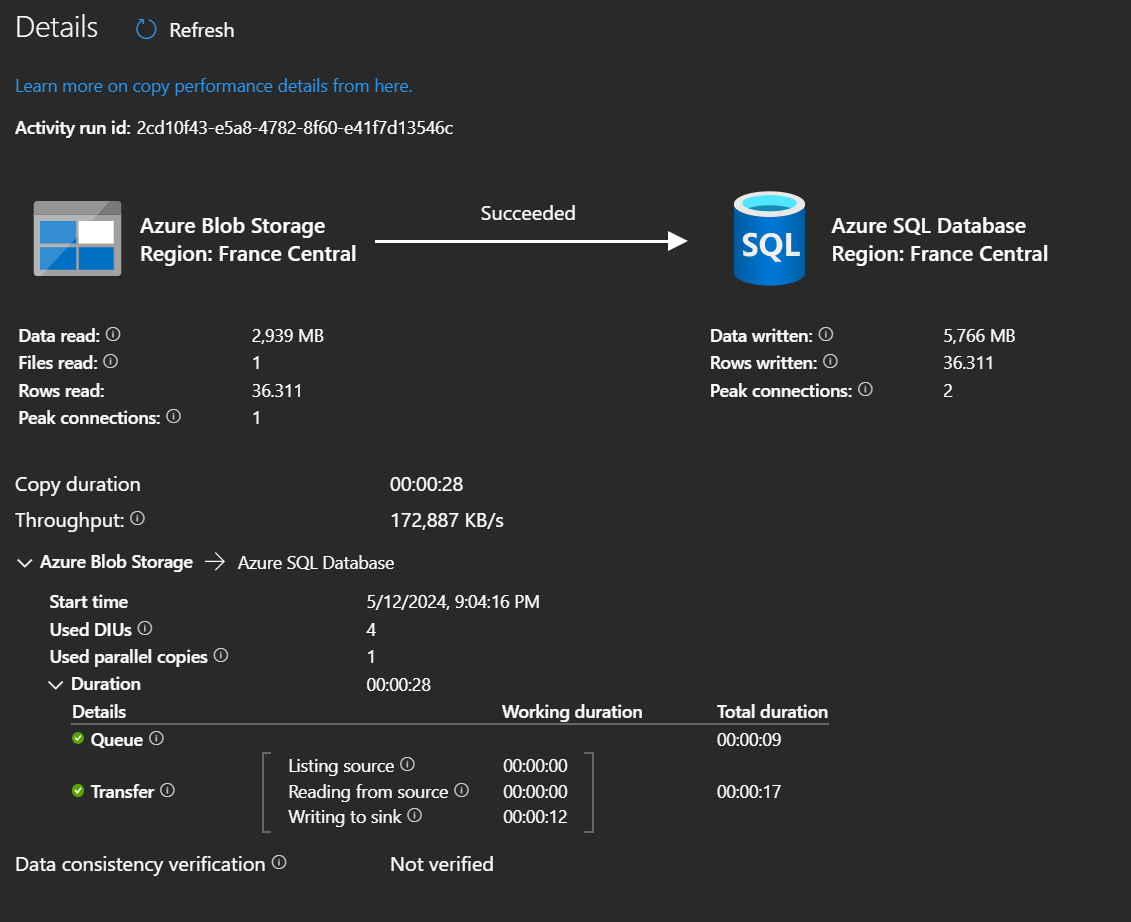
\includegraphics[scale = 0.4]{imgs/move_data_squema.png}
    \caption{Esquema de la Copy Activity realizada.}
    \label{DataFactory}
\end{figure}

\B{Esta actividad se ha configurado para que se realice de manera concurrente diariamente}. Es decir, hay otra capa de automatización en el proyecto.

\subsubsection{SQL Server}
Hasta ahora se ha hablado de Azure SQL Database pero no de Azure SQL Server. La función de Azure SQL Server es gestionar y alojar una o incluso varias bases de datos SQL (en el caso de este trabajo una). Otra utilidad muy importante que proporciona un \ti{endpoint} para poder conectarse a la base de datos; tanto desde Azure Data Factory, como desde SQL Server Management Studio, como desde Power BI. Véase la Figura \ref{serverEndpoint}.

\begin{figure}[H]
    \centering
    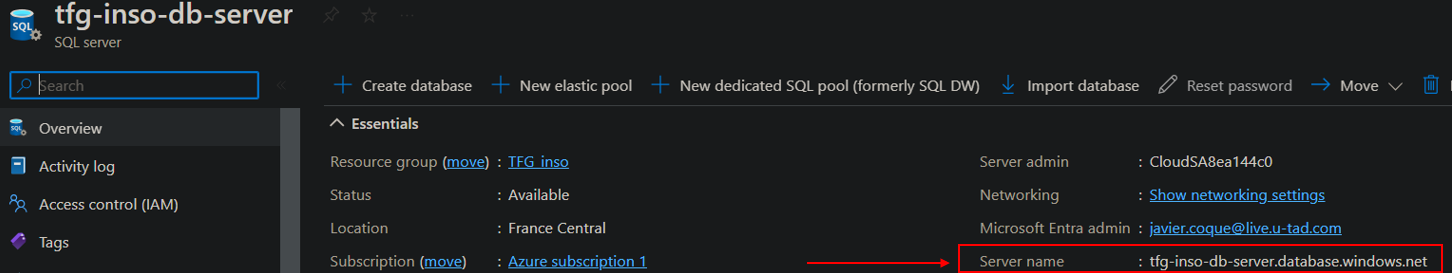
\includegraphics[width = 0.9\textwidth]{imgs/serverEndpoint.png}
    \caption{SQL Server endpoint.}
    \label{serverEndpoint}
\end{figure}

Por último, y no por ello menos importante, mencionar el uso de la herramienta ---ya mencionada con anterioridad--- SQL Server Management Studio. Con ella y comandos básicos de SQL se ha creado un usuario, y la tabla en bases datos para el proyecto. Para más información de los comandos empleados en Github ir a Desarrollo/SQL\_scripts.

\begin{nota}
    Para no alargar en exceso este apartado  se dejan referencias de configuración de todo lo mencionado hasta ahora: Azure Data Factory, Azure Blob Storage, etc. Para más información, por favor diríjase al \href{https://github.com/JCOQUE/TFG-ingenieria/blob/main/README.md}{README.md} de Github en la sección \ti{Tools/Azure}.
    \begin{itemize}
        \item Documentación extra-oficial: \parencite{azure1}, \parencite{azure2}, \parencite{azure3}, \parencite{azure4}, \parencite{azure5}, \parencite{azure6}.
    \end{itemize}
\end{nota}

Una vez los  datos ya están en el lugar desde donde Power BI los extraerá, únicamente queda recogerlos y mostrarlos.

\subsection{Visualización de los datos}
Para la visualización de los datos se  ha empleado la herramienta de Power BI por su sencillez y su interactividad entre gráficas. Con esta herramienta se ha realizado el \ti{dashboard} final. Véase la \ref{PowerBI} para posicionar esta  herramienta dentro de la arquitectura del proyecto mostrada en la Figura \ref{arquitectura}.

\begin{figure}[H]
    \centering
    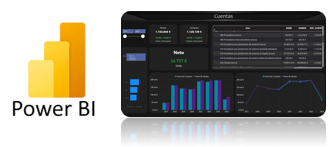
\includegraphics{imgs/powerBI.png}
    \caption{Última sección de la arquitectura del proyecto: Power BI.}
    \label{PowerBI}
\end{figure}

Power BI se conecta a tres fuentes de datos: la tabla SQL mencionada en el apartado anterior y dos Excel adicionales para aportar cierta inteligencia temporal y de cuentas contables (\Code{Calendario} y \Code{PGC} respectivamente). Esto es, por ejemplo, para ordenar los meses correctamente en los datos (Power BI los ordena alfabéticamente: abril, agosto, etc.). Respecto a las cuentas bancarias, para poder relacionar la cuenta 100 con Financiación Básica y demás.

Para añadir dinamismo a las gráficas y que el usuario tenga cierto control sobre qué gráficas quiere ver, se han introducido lo que Power BI llama como \ti{parámetros}. Además, para poder sacarle provecho a los datos, se han incluido lo que Power BI llama \ti{medidas} para obtener ciertos resultados deseados a partir de los datos existentes. Estas medidas están escritas en código DAX (\ti{Data Analysis Expressions}). Para poder ver mejor cómo están relacionadas unas tablas con otras y los parámetros utilizados, véase la Figura \ref{esquemaPowerBI}.

\begin{figure}[H]
    \centering
    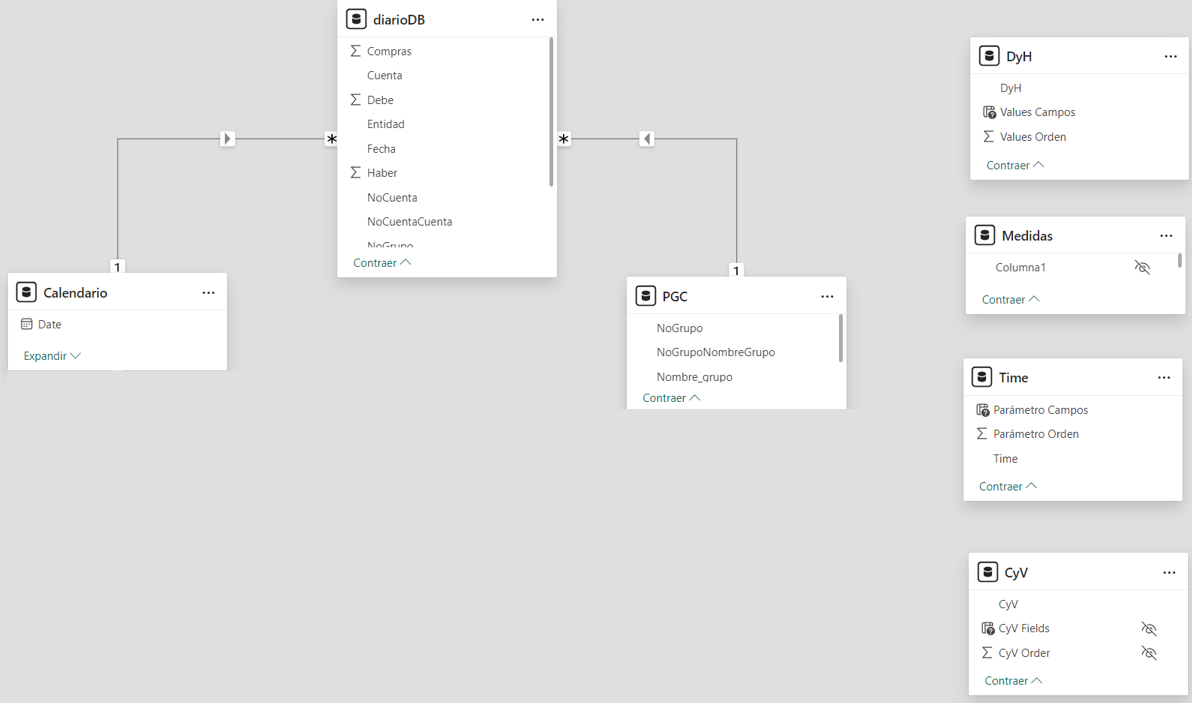
\includegraphics[width = 0.9\textwidth]{imgs/esquemaPowerBI.png}
    \caption{Esquema relacional Power BI.}
    \label{esquemaPowerBI}
\end{figure}

En la Figura \ref{esquemaPowerBI} se  muestran cuatro tablas: \Code{diarioDB}, \Code{Calendario},\Code{PGC} y \Code{Medidas}. Esta última se trata de una tabla \ti{dummy} que contiene una columna vacía. Esto es una práctica común en Power BI, con el único objetivo de tener todas las medidas creadas con DAX en una misma tabla ---y así no tenerlas repartidas por distintas tablas---. Además, en la Figura \ref{esquemaPowerBI} se puede ver cómo las tablas \Code{Calendario} y \Code{PGC} están relacionadas con la tabla \Code{diarioDB}. Por ser un poco más concretos, la tabla \Code{Calendario} está relacionada con la columna \ti{Time} de \Code{diarioDB}, mientras que la tabla \Code{PGC} con la columna \ti{NoGrupo}.


\subsubsection{Actualización incremental}
La actualización incremental ---o \ti{incremental refreshing} en inglés--- es una característica que ofrece Power BI para únicamente actualizar datos nuevos. Los datos clasificados como nuevos se definen en una política de configuración de la propia actualización incremental. Esta  característica, en un entorno \ti{Big Data} con una inmensa cantidad de datos, es \B{esencial}. 

El exclusivo motivo por el que se ha decidido \B{implementar una base de datos SQL} en el desarrollo de este trabajo es porque para poder hacer una \B{actualización incremental}, el sistema de alojamiento desde donde Power BI extrae los datos a utilizar, debe permitir una operación llamada \ti{query folding}. Esta operación se trata de una técnica de optimización en el contexto ETL (Extracción, Transformación y Carga de datos), en la que el filtrado de datos se hace en el sistema de origen en lugar de en el sistema de alimentación. Es decir, que el filtrado de datos que se pueda realizar como consecuencia de la actualización incremental, se hace ---en el caso de este trabajo--- en la tabla SQL, en lugar de en Power BI. Esta operación no está soportada por todos los sistemas de almacenamiento de datos; pero por bases de datos SQL sí.

Para realizar una actualización incremental sobre una tabla de Power BI, hay que definir previamente unos parámetros de tiempo en una columna de tipo \ti{Time} en la tabla \Code{diarioDB} para el caso concreto de este trabajo \parencite{incrRefr}. Una vez hecho esto, se puede proceder configurar esta actualización incremental. Véase la Figura \ref{refreshPolicy}.

\begin{figure}[H]
    \centering
    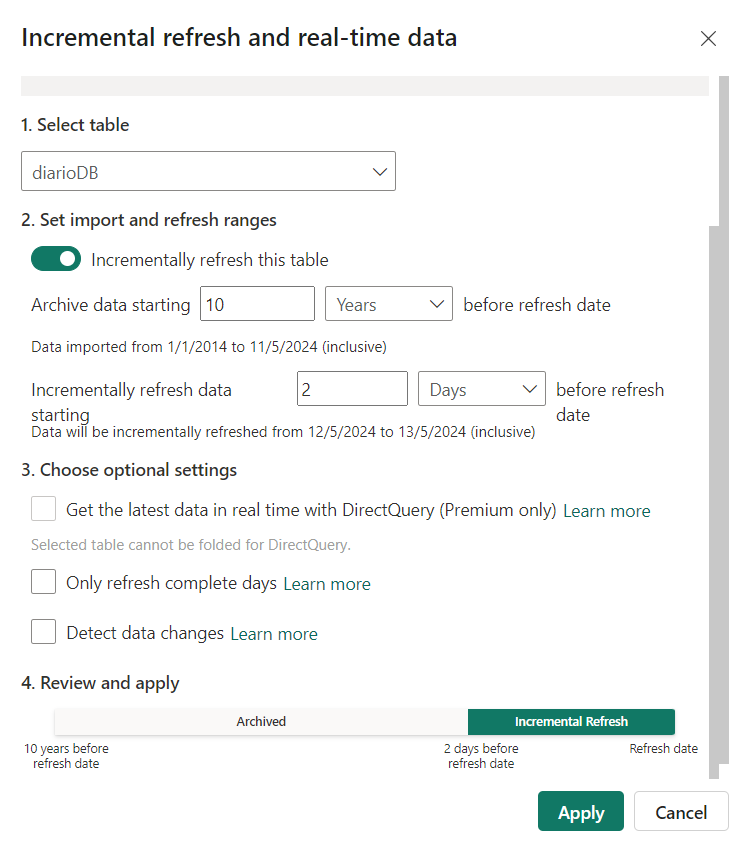
\includegraphics[scale = 0.6]{imgs/refresh_policy.png}
    \caption{Política de configuración de actualización incremental.}
    \label{refreshPolicy}
\end{figure}

En la Figura \ref{refreshPolicy}, justo encima de los botones \ti{Apply} y \ti{Cancel} se puede entender muy bien la configuración establecida. Se van a leer datos de los últimos diez años y a cargar únicamente aquellos datos que se hayan modificado en los últimos dos días; manteniendo el resto de datos intactos. Esta configuración, en un entorno real debería configurarse según la situación, tipo de datos, arquitectura implementada, etc.

\subsubsection{Resultado final}

\label{resFinal}
El resultado final son cuatro pestañas; cada una con un \ti{dashboard} distinto. El primer \ti{dashboard} es uno general que, adicionalmente a las tablas mencionadas con anterioridad, hace uso del parámetro \Code{CyV} mostrado en la Figura \ref{esquemaPowerBI}. El parámetro \Code{CyV} permite al usuario que decida sobre si las gráficas muestran información de Compras o de Ventas de la empresa. Véase la Figura \ref{general}.

\begin{figure}[H]
	\centering
	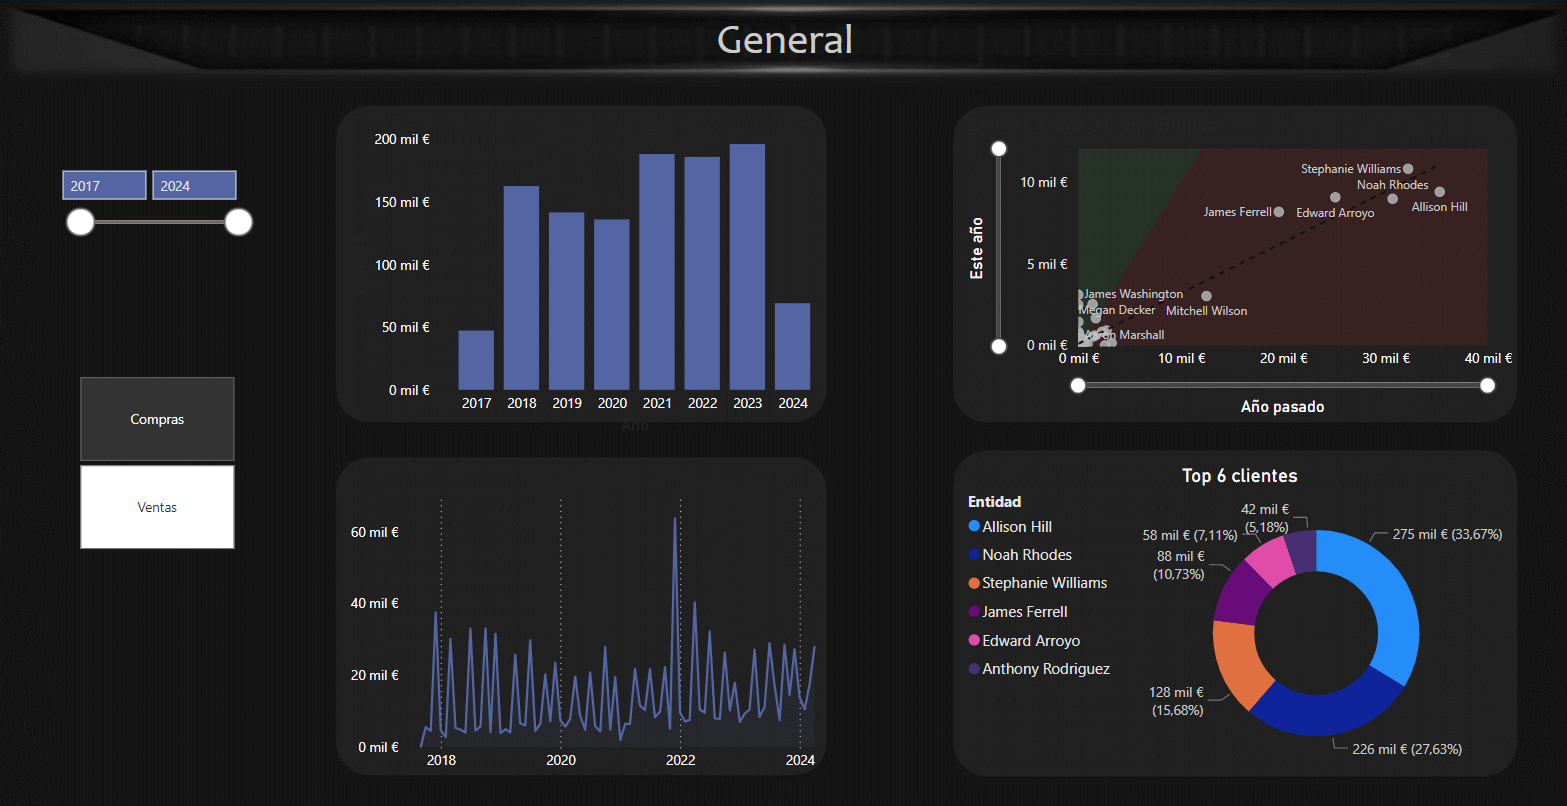
\includegraphics[width= 0.8\textwidth]{imgs/general_dashboard}
	\caption{Pestaña General dashboard.}
	\label{general}
\end{figure}

En la Figura \ref{general} se trata de mostrar un \ti{dashboard} general con información respecto a Compras o Ventas;  algo que se puede especificar en los botones de la izquierda. Además de esto, el usuario también puede elegir entre el periodo de tiempo que más le interese. El color del \ti{dashboard} elegido es \B{negro}, pues añade elegancia y simplicidad a las gráficas.

En cuanto a las gráficas, se ha optado por elegir dos clásicas, de barras y de línea, para mostrar el parámetro seleccionado por el usuario de manera cuantitativa. Adicionalmente a estas gráficas, se ha considerado interesante mostrar una gráfica de tipo \ti{scatter} en la que se comparen las Compras o Ventas de los clientes un año en concreto, con respecto al año anterior. De esta manera, se puede ver si un año dado está haciendo clientes a los que se está comprando o vendiendo en mayor o menor cantidad que respecto al año anterior. Esta gráfica ayuda de manera sustancial para tener un mejor seguimiento de los clientes, por si hubiera que llamar a alguno de ellos ---o cualquier otra razón comercial que va más allá en este trabajo---. También los ejes de esta gráfica son modificables por el usuario. Por último, abajo a la derecha, se muestra una gráfica de tarta mostrando los \ti{Top 6 clientes} del respectivo parámetro. De nuevo, por motivos comerciales principalmente, pero también para otros muchos ámbitos de la empresa.


El segundo \ti{dashboard} ofrece una comparativa entre Compras y Ventas, así como una comparativa de cada una de estas medidas respecto al año pasado hasta el día actual. Por último, ofrece una visión rápida y eficaz de todas las diferentes cuentas, su Debe y Haber, para cada año. De esta manera, si el método de la partida doble se hubiera empleado mal en algún momento, es muy fácil de ver. Véase la Figura \ref{cuentas} en donde se muestra este segundo \ti{dashboard}.


\begin{figure}[H]
	\centering
	\includegraphics[width= 0.8\textwidth]{imgs/cuentas_dashboard}
	\caption{Pestaña Cuentas dashboard.}
	\label{cuentas}
\end{figure}

En la pestaña de la Figura \ref{cuentas} el usuario también puede elegir una ventana temporal sobre la que mostrar los datos contables. Además, abajo a la izquierda, se muestra una gráfica de preguntas y respuestas. Esta gráfica hace uso de inteligencia artificial incorporada por Power BI para tratar de resolver preguntas acerca de los datos. Arriba a la derecha de esta gráfica, se encuentran 3 tarjetas mostrando información acerca de Compras, Ventas y neto. Las dos primeras muestran adicionalmente una comparativa entre las Compras y Ventas del máximo año seleccionado respecto al año anterior. Esta comparativa es interesante porque, en caso de que se haga del año actual con respecto al año anterior, se tiene en cuenta el día del actual año para la comparativa con el año previo\fnm. Las dos gráficas inferiores, al igual que en la  pestaña anterior, son gráficas de barras y línea. La diferencia radica en que estas gráficas muestran las dos variables a la vez, permitiendo una comparativa entre ellas de una manera mucho más clara y efectiva. Por último, arriba a la derecha, se encuentra la gráfica más importante de este \ti{dashboard}: la gráfica que muestra información de Debe y Haber de las cuentas contables de cada año. Esta gráfica es de inmensa utilidad para un contable, pues muestra de manera muy clara si se está cumpliendo con el método de la partida doble de contabilidad. Este, como se mencionó en la sección 2, es un principio fundamental de la contabilidad y debe cumplirse \B{siempre}.

\fnt{De esta manera,  si se está a ocho de agosto, realiza una comparativa hasta el ocho de agosto del año pasado. Esto permite una comparación ``limpia" entre dos años si uno de ellos no ha terminado todavía.}



El tercer \ti{dashboard} utiliza gráficas de análisis avanzado no propias de Power BI, sino de Zebra BI. Este \ti{dashboard} es el menos llamativo estéticamente debido a que la versión gratuita de Zebra BI ofrece pocas posibilidades de cambiar la estética de las gráficas. Aun así, las  gráficas mostradas en esta pestaña ofrecen un análisis muy potente. Por un lado, las cuentas contables de un año en concreto con respecto al año previo, dejando al usuario elegir entre Debe y Haber con el parámetro \Code{DyH} y la estacionalidad con el parámetro \Code{Time} (Figura \ref{esquemaPowerBI}). Por otro lado, en las Compras y Ventas (según determine el usuario) y, de nuevo, con respecto al año previo a partir de un año seleccionado. Véase la Figura \ref{analisis}.

\begin{figure}[H]
	\centering
	\includegraphics[width= 0.8\textwidth]{imgs/analisis_dashboard}
	\caption{Pestaña Análisis dashboard.}
	\label{analisis}
\end{figure}

En la Figura \ref{analisis} se pueden ver las dos gráficas mencionadas anteriormente. También, se permite al usuario elegir el año sobre el que este quiere que le muestre la información. Esto, teniendo en cuenta que ambas gráficas mostradas realizarán una comparativa entre el año seleccionado y el anterior. Además, una característica importante de la gráfica de la derecha en la Figura \ref{analisis}, es que cuenta con un botón (solo se ve al pasar el ratón por encima) que permite mostrar otro tipo de gráficas analíticas.

Ambos gráficos de Zebra BI mostrados en este \ti{dashboard} son muy potentes analítica y comparativamente. Estos gráficos son los más  utilizados, por empresas que utilizan Power BI, a nivel de finanzas y ventas \parencite{zebraBI}. Este trabajo está restringido ---a nivel de estética, pero sobre todo de aporte de mayor información--- a que estas gráficas son de pago. De esta manera, modificarlas y obtener más información acerca de ellas, es una tarea que va más allá del contenido de este trabajo.

Por último, está el \ti{dashboard} de BA que contiene las predicciones comentadas en el apartado \ti{Comparativa de modelos} de esta misma sección del trabajo. Esta pestaña ofrece información acerca de las previsiones de compras y ventas en los siguientes tres meses por parte de la empresa. Esto es fundamental porque se puede prever un aumento de compras en los siguientes meses y que la empresa no tenga suficiente liquidación y tenga que anticiparse a la situación, ya sea con pagarés, adelantando el cobro a clientes que habían pagado con una letra, pedir un préstamo al banco, etc. Tener datos futuros permite a la empresa anticiparse a las distintas situaciones, yendo siempre un paso por delante. Véase la Figura \ref{predicciones}.

\begin{figure}[H]
	\centering
	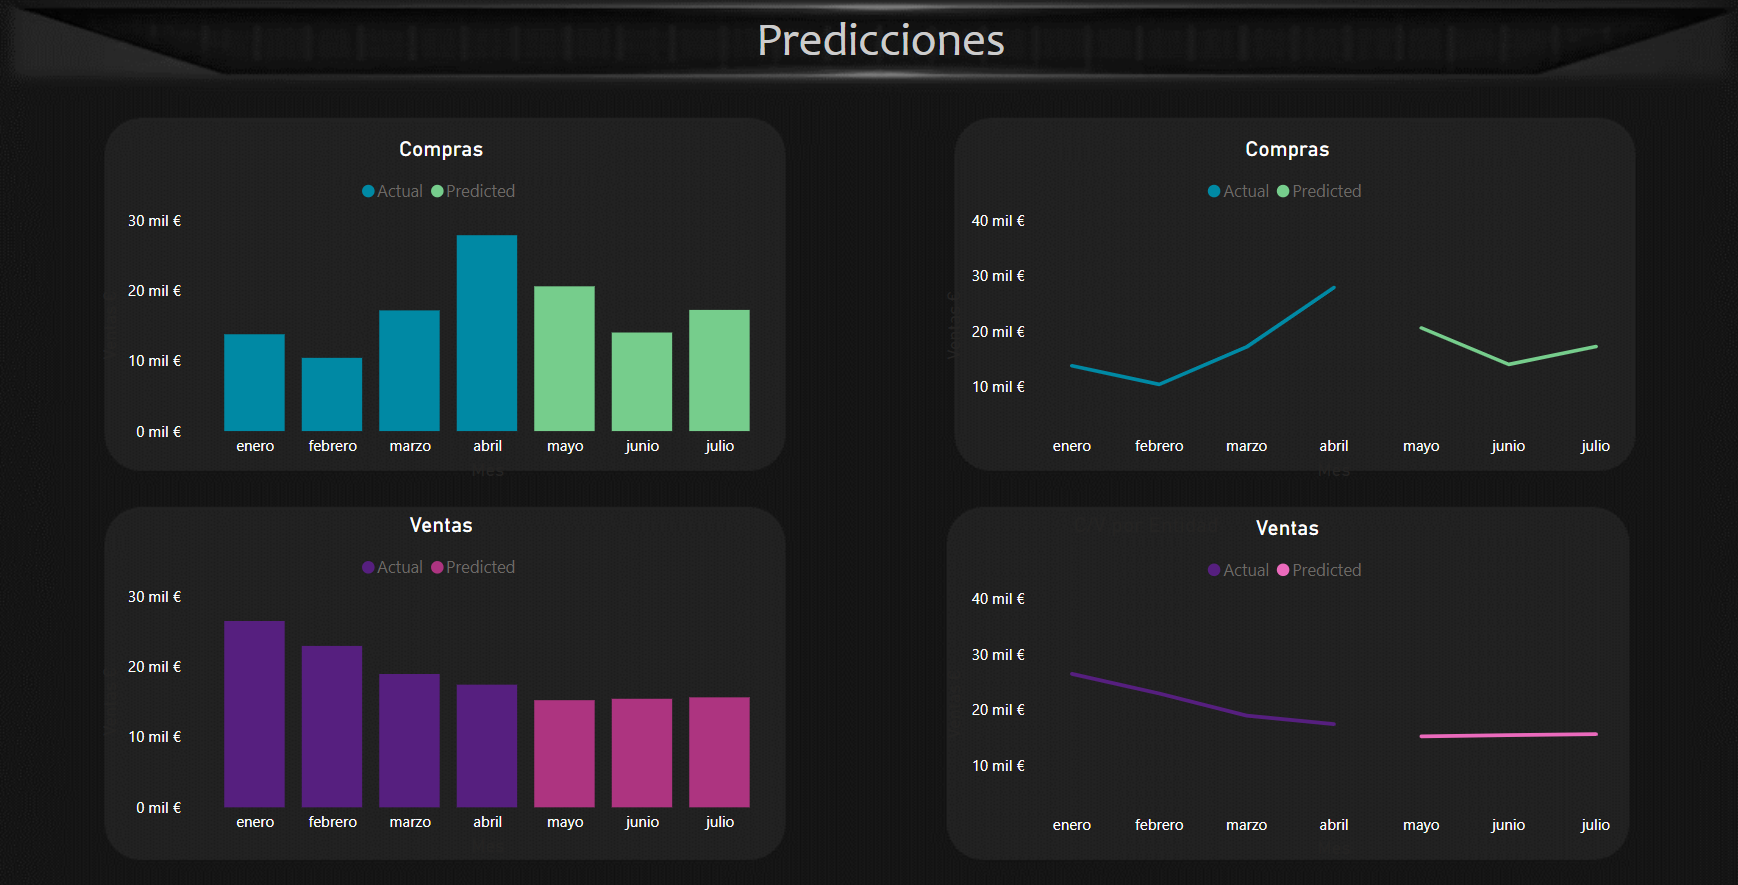
\includegraphics[width= 0.8\textwidth]{imgs/predicciones_dashboard}
	\caption{Pestaña Predicciones dashboard.}
	\label{predicciones}
\end{figure}

Todos estos \ti{dashboard} tienen en común que son \B{totalmente interactivos} y fáciles de usar. Además cuentan  con características adicionales propias de Power BI muy interesantes, pero que no son mencionadas en este apartado por no ser un tema principal.

Para terminar, se ha visto interesante crear un diseño para móviles y publicarlo para que el \ti{dashboard} pueda ser visualizado desde el teléfono móvil. De esta manera, se consigue que el\ti{dashboard} sea más accesible, pudiéndolo consultar en un ámbito fuera de la oficina. Véase la Figura \ref{PBImovil}.

\begin{figure}[H]
	\centering
	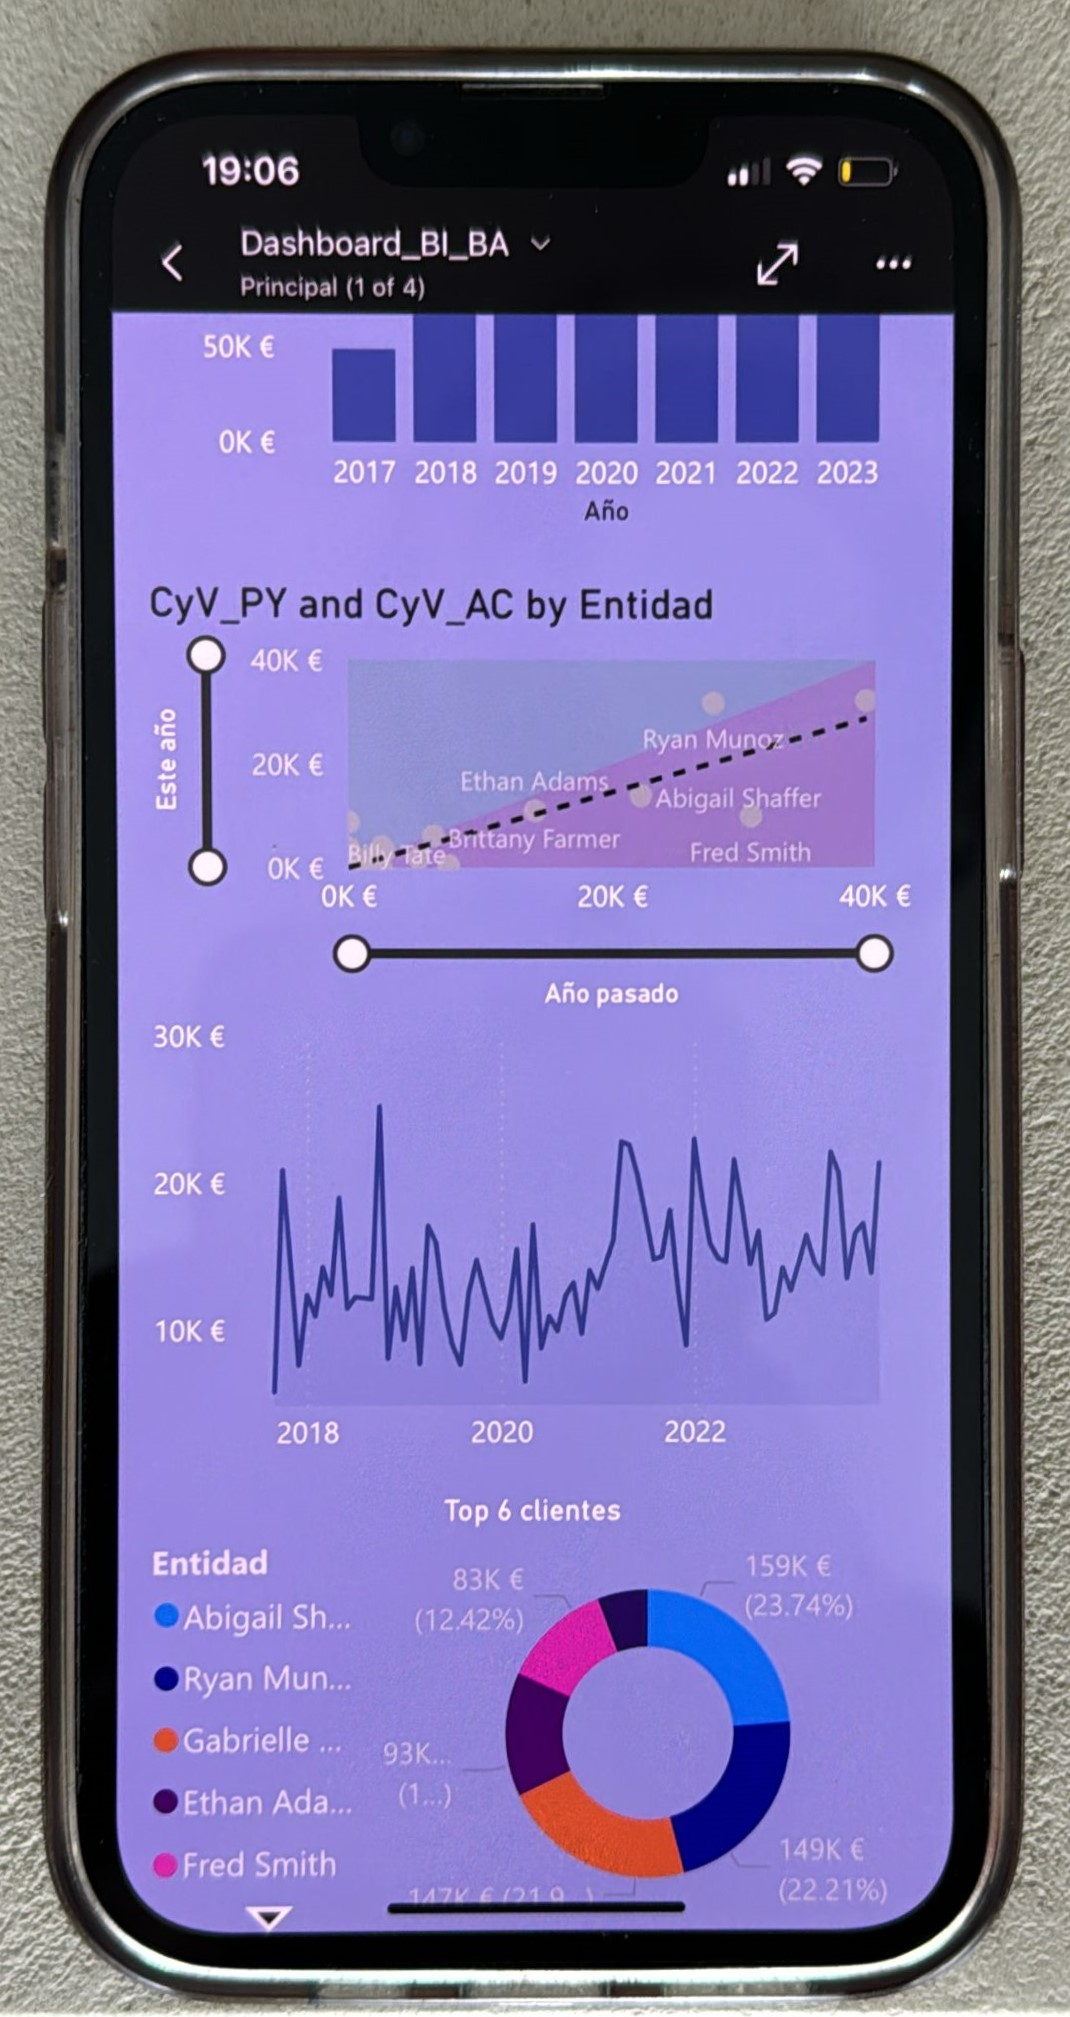
\includegraphics[scale =  0.2]{imgs/PBImovil.jpeg}
	\caption{Resultado final del proyecto en teléfono móvil personal.}
	\label{PBImovil}
\end{figure}


\subsubsection{Publicación del dashboard en la nube}
Suponiendo que se está trabajando en un entorno colaborativo con más personas o, que simplemente se quiere que las personas puedan ver el \ti{dashboard} sin necesidad de mandárselo explícitamente cada vez que lo necesiten, se ha publicado el \ti{dashboard} en la nube en un entorno de trabajo en el que estarían las personas interesadas y/o involucradas en el \ti{dashboard}. Esta característica, junto con la posibilidad de ver del \ti{dashboard} desde un teléfono móvil, convierte a esta aplicación lo más accesible posible.

Para hacer esto, es tan sencillo como darle al botón de "Publicar" en Power BI. Pero, si se quiere que desde la nube se actualicen los datos sin que uno tenga que hacerlo desde local, hay que configurar unos \ti{gateways} que se conecten desde el servidor hasta las fuentes de datos para poder actualizarlos desde la nube. En el caso particular de este trabajo, hay dos \ti{gateways}: uno hacia el ordenador del autor (para las  tablas \Code{Calendario} y \Code{PGC}, mencionadas con anterioridad) y otra hacia la base de datos SQL para la tabla \Code{diarioDB}. Para  ello, una vez en la nube, uno debe dirigirse al modelo semántico del \ti{dashboard} (cuando se publica un \ti{dashboard} en la nube se crea automáticamente el modelo semántico que son los  datos en sí y el reporte que es el \ti{dashboard}), tres puntos y ajustes. Una vez hecho esto, en la sección de \ti{Gateways and cloud connections} se configuran.
Véase la Figura \ref{PBIgateways}.

\begin{figure}[H]
    \centering
    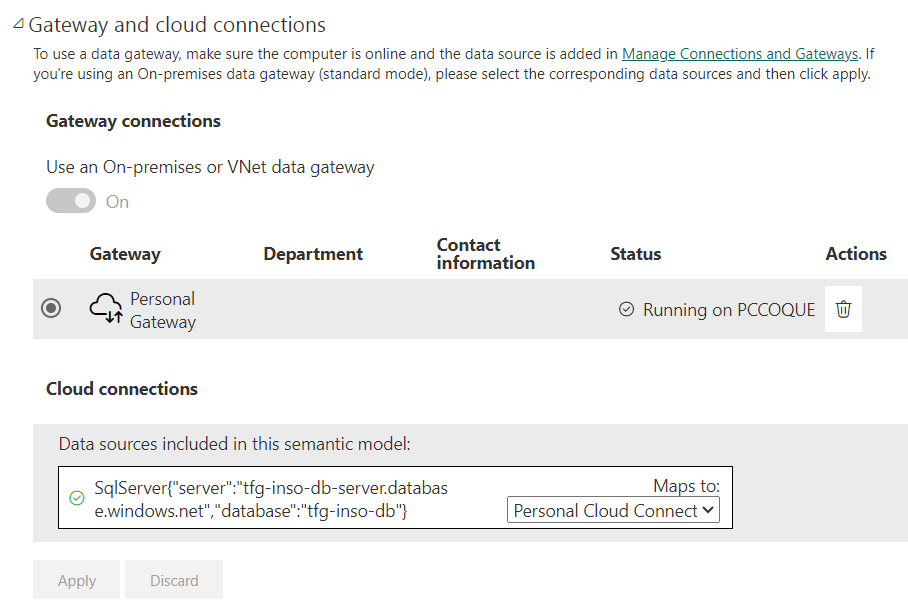
\includegraphics[scale = 0.7]{imgs/PBIgateways.png}
    \caption{Gateways creadas en el servidor de Power BI.}
    \label{PBIgateways}
\end{figure}



